% Options for packages loaded elsewhere
\PassOptionsToPackage{unicode}{hyperref}
\PassOptionsToPackage{hyphens}{url}
%
\documentclass[
]{book}
\usepackage{amsmath,amssymb}
\usepackage{iftex}
\ifPDFTeX
  \usepackage[T1]{fontenc}
  \usepackage[utf8]{inputenc}
  \usepackage{textcomp} % provide euro and other symbols
\else % if luatex or xetex
  \usepackage{unicode-math} % this also loads fontspec
  \defaultfontfeatures{Scale=MatchLowercase}
  \defaultfontfeatures[\rmfamily]{Ligatures=TeX,Scale=1}
\fi
\usepackage{lmodern}
\ifPDFTeX\else
  % xetex/luatex font selection
\fi
% Use upquote if available, for straight quotes in verbatim environments
\IfFileExists{upquote.sty}{\usepackage{upquote}}{}
\IfFileExists{microtype.sty}{% use microtype if available
  \usepackage[]{microtype}
  \UseMicrotypeSet[protrusion]{basicmath} % disable protrusion for tt fonts
}{}
\makeatletter
\@ifundefined{KOMAClassName}{% if non-KOMA class
  \IfFileExists{parskip.sty}{%
    \usepackage{parskip}
  }{% else
    \setlength{\parindent}{0pt}
    \setlength{\parskip}{6pt plus 2pt minus 1pt}}
}{% if KOMA class
  \KOMAoptions{parskip=half}}
\makeatother
\usepackage{xcolor}
\usepackage{color}
\usepackage{fancyvrb}
\newcommand{\VerbBar}{|}
\newcommand{\VERB}{\Verb[commandchars=\\\{\}]}
\DefineVerbatimEnvironment{Highlighting}{Verbatim}{commandchars=\\\{\}}
% Add ',fontsize=\small' for more characters per line
\usepackage{framed}
\definecolor{shadecolor}{RGB}{248,248,248}
\newenvironment{Shaded}{\begin{snugshade}}{\end{snugshade}}
\newcommand{\AlertTok}[1]{\textcolor[rgb]{0.94,0.16,0.16}{#1}}
\newcommand{\AnnotationTok}[1]{\textcolor[rgb]{0.56,0.35,0.01}{\textbf{\textit{#1}}}}
\newcommand{\AttributeTok}[1]{\textcolor[rgb]{0.13,0.29,0.53}{#1}}
\newcommand{\BaseNTok}[1]{\textcolor[rgb]{0.00,0.00,0.81}{#1}}
\newcommand{\BuiltInTok}[1]{#1}
\newcommand{\CharTok}[1]{\textcolor[rgb]{0.31,0.60,0.02}{#1}}
\newcommand{\CommentTok}[1]{\textcolor[rgb]{0.56,0.35,0.01}{\textit{#1}}}
\newcommand{\CommentVarTok}[1]{\textcolor[rgb]{0.56,0.35,0.01}{\textbf{\textit{#1}}}}
\newcommand{\ConstantTok}[1]{\textcolor[rgb]{0.56,0.35,0.01}{#1}}
\newcommand{\ControlFlowTok}[1]{\textcolor[rgb]{0.13,0.29,0.53}{\textbf{#1}}}
\newcommand{\DataTypeTok}[1]{\textcolor[rgb]{0.13,0.29,0.53}{#1}}
\newcommand{\DecValTok}[1]{\textcolor[rgb]{0.00,0.00,0.81}{#1}}
\newcommand{\DocumentationTok}[1]{\textcolor[rgb]{0.56,0.35,0.01}{\textbf{\textit{#1}}}}
\newcommand{\ErrorTok}[1]{\textcolor[rgb]{0.64,0.00,0.00}{\textbf{#1}}}
\newcommand{\ExtensionTok}[1]{#1}
\newcommand{\FloatTok}[1]{\textcolor[rgb]{0.00,0.00,0.81}{#1}}
\newcommand{\FunctionTok}[1]{\textcolor[rgb]{0.13,0.29,0.53}{\textbf{#1}}}
\newcommand{\ImportTok}[1]{#1}
\newcommand{\InformationTok}[1]{\textcolor[rgb]{0.56,0.35,0.01}{\textbf{\textit{#1}}}}
\newcommand{\KeywordTok}[1]{\textcolor[rgb]{0.13,0.29,0.53}{\textbf{#1}}}
\newcommand{\NormalTok}[1]{#1}
\newcommand{\OperatorTok}[1]{\textcolor[rgb]{0.81,0.36,0.00}{\textbf{#1}}}
\newcommand{\OtherTok}[1]{\textcolor[rgb]{0.56,0.35,0.01}{#1}}
\newcommand{\PreprocessorTok}[1]{\textcolor[rgb]{0.56,0.35,0.01}{\textit{#1}}}
\newcommand{\RegionMarkerTok}[1]{#1}
\newcommand{\SpecialCharTok}[1]{\textcolor[rgb]{0.81,0.36,0.00}{\textbf{#1}}}
\newcommand{\SpecialStringTok}[1]{\textcolor[rgb]{0.31,0.60,0.02}{#1}}
\newcommand{\StringTok}[1]{\textcolor[rgb]{0.31,0.60,0.02}{#1}}
\newcommand{\VariableTok}[1]{\textcolor[rgb]{0.00,0.00,0.00}{#1}}
\newcommand{\VerbatimStringTok}[1]{\textcolor[rgb]{0.31,0.60,0.02}{#1}}
\newcommand{\WarningTok}[1]{\textcolor[rgb]{0.56,0.35,0.01}{\textbf{\textit{#1}}}}
\usepackage{longtable,booktabs,array}
\usepackage{calc} % for calculating minipage widths
% Correct order of tables after \paragraph or \subparagraph
\usepackage{etoolbox}
\makeatletter
\patchcmd\longtable{\par}{\if@noskipsec\mbox{}\fi\par}{}{}
\makeatother
% Allow footnotes in longtable head/foot
\IfFileExists{footnotehyper.sty}{\usepackage{footnotehyper}}{\usepackage{footnote}}
\makesavenoteenv{longtable}
\usepackage{graphicx}
\makeatletter
\def\maxwidth{\ifdim\Gin@nat@width>\linewidth\linewidth\else\Gin@nat@width\fi}
\def\maxheight{\ifdim\Gin@nat@height>\textheight\textheight\else\Gin@nat@height\fi}
\makeatother
% Scale images if necessary, so that they will not overflow the page
% margins by default, and it is still possible to overwrite the defaults
% using explicit options in \includegraphics[width, height, ...]{}
\setkeys{Gin}{width=\maxwidth,height=\maxheight,keepaspectratio}
% Set default figure placement to htbp
\makeatletter
\def\fps@figure{htbp}
\makeatother
\setlength{\emergencystretch}{3em} % prevent overfull lines
\providecommand{\tightlist}{%
  \setlength{\itemsep}{0pt}\setlength{\parskip}{0pt}}
\setcounter{secnumdepth}{5}
\usepackage{booktabs}
\ifLuaTeX
  \usepackage{selnolig}  % disable illegal ligatures
\fi
\usepackage[]{natbib}
\bibliographystyle{plainnat}
\IfFileExists{bookmark.sty}{\usepackage{bookmark}}{\usepackage{hyperref}}
\IfFileExists{xurl.sty}{\usepackage{xurl}}{} % add URL line breaks if available
\urlstyle{same}
\hypersetup{
  pdftitle={Introduction to evolutionary and coevolutionary theory},
  pdfauthor={Leandro G. Cosmo},
  hidelinks,
  pdfcreator={LaTeX via pandoc}}

\title{Introduction to evolutionary and coevolutionary theory}
\author{Leandro G. Cosmo}
\date{2024-07-22}

\begin{document}
\maketitle

{
\setcounter{tocdepth}{1}
\tableofcontents
}
\hypertarget{preface}{%
\chapter{Preface}\label{preface}}

Coevolution, the reciprocal evolutionary influence between two or more interacting species, underpins the diversity and complexity of ecosystems. However, understanding coevolution in empirical systems is challenging because of the different time scales at which coevolution operates. Mathematical models, in turn, enable us to simulate various scenarios, predict outcomes, and test hypotheses, providing a deeper understanding of how coevolution shapes biodiversity, ecological stability, and the emergence of new traits. Therefore, the main goal of the course is to introduce the basic concepts and tools that can be used to model coevolution in ecological communities. To do so, the course is divided into two blocks. In the first block, we will introduce the main concepts and the mathematical foundations of evolutionary biology that will be used to model coevolution. For the second block we will provide an overview on how to build coevolutionary models from basic evolutionary and ecological principles. The coevolutionary models covered in the course can be applied to both discrete and continuously varying traits, for instance, the frequency of different flower color morphs in a population of plants or the length of their floral tube, respectively. Furthermore, we will demonstrate how to progress the coevolutionary models from isolated pairwise of interacting species to entire communities that form networks. Conceptual lectures will occur in the morning, from 10:00-12:00am. The conceptual lectures will be followed by an exercise section in the afternoon, from 14:00-17:00pm, where the models will be implemented via computer simulations and analyzed.

At a future date this page will be updated to include the lecture notes, as well as the instructions for the exercise sections of each of the lectures. If you have any questions, please feel free to send me an e-mail. I will be happy to help!

\hypertarget{registration}{%
\section{Registration}\label{registration}}

For the present iteration of the course, registration will take place between \textbf{10.06.2024} and \textbf{27.06.2024}. The Ecology graduate program of Universidade Estadual de Campinas requires students to register using the following forms:

\begin{enumerate}
\def\labelenumi{\arabic{enumi})}
\tightlist
\item
  \href{https://drive.google.com/file/d/1fRILwlcdKFloCCqvmGSjI9ucSElKDnaJ/view}{``Estudantes regulares''} - for students of the Ecology graduate program of Universidade Estadual de Campinas
\item
  \href{https://www.dac.unicamp.br/sistemas/formularios/inscricao_disciplinas_eventuais_pos_aut.php}{``Estudantes especiais''} - for students of different programs or institutions.
\end{enumerate}

Please, fill the appropriate form and send it to the email \href{mailto:leandro.giacobellicosmo@uzh.ch}{\nolinkurl{leandro.giacobellicosmo@uzh.ch}} with the subject ``Course pre-registration''. Even though this page and course notes are in english, \textbf{all of the lectures of the course will be in Portuguese.} The course will award 2 credits.

\hypertarget{course-schedule}{%
\section{Course schedule}\label{course-schedule}}

All of the lectures of the course will be held \textbf{in-person}, at the Instituto de Biologia of the Universidade Estadual de Campinas. Throughout the two blocks of the course we will study the following topics:

\textbf{Block 1 -- Evolution by natural selection and the fundamental equations of evolutionary theory}

\begin{enumerate}
\def\labelenumi{\arabic{enumi})}
\tightlist
\item
  Introduction to the course: why do we need evolution and coevolution to understand ecological communities?
\item
  Wright's equation for the adaptive landscape of genotypes.
\item
  The algebra of evolution -- Price's theorem and the different modes of selection.
\item
  Lande's equation, the selection gradient, and the adaptive landscape of phenotypes.
\end{enumerate}

\textbf{Block 2 - Ecological interactions as reciprocal selective pressures: coevolution in ecological communities}

\begin{enumerate}
\def\labelenumi{\arabic{enumi})}
\tightlist
\item
  Coevolution of discrete morphs/haploid individuals: ecological interactions mediated by a gene-for-gene or matching allele mechanism.
\item
  Coevolution of continuously varying traits: when trait matching, and exploitation barriers mediate the outcome of ecological interactions.
\item
  Coevolution in species-rich ecological communities: the role of indirect evolutionary effects.
\end{enumerate}

The day-to-day schedule can be found below:

\textbf{Lectures of the first block:}

\begin{longtable}[]{@{}
  >{\centering\arraybackslash}p{(\columnwidth - 6\tabcolsep) * \real{0.0718}}
  >{\centering\arraybackslash}p{(\columnwidth - 6\tabcolsep) * \real{0.3591}}
  >{\centering\arraybackslash}p{(\columnwidth - 6\tabcolsep) * \real{0.3149}}
  >{\centering\arraybackslash}p{(\columnwidth - 6\tabcolsep) * \real{0.2486}}@{}}
\toprule\noalign{}
\begin{minipage}[b]{\linewidth}\centering
\end{minipage} & \begin{minipage}[b]{\linewidth}\centering
Day 1 (16.07.2024)
\end{minipage} & \begin{minipage}[b]{\linewidth}\centering
Day 2 (17.07.2024)
\end{minipage} & \begin{minipage}[b]{\linewidth}\centering
Day 3 (18.07.2024)
\end{minipage} \\
\midrule\noalign{}
\endhead
\bottomrule\noalign{}
\endlastfoot
Morning lecture

(from 10:00 to 12:00am) & Introduction to the course and how can we model evolutionary changes in the frequencies of morphs (Wright's adaptive landscape) & The algebra of evolution - Price's theorem and the different modes of selection & Modelling the evolution of continuous traits - Lande's equation and selection gradients \\
Exercise section

(from 14:00 to 16:00pm) & Using simulations to understand the evolution and adaptive landscape of discrete morphs & Using the Price equation and linear regressions to understand directional, stabilizing and disruptive selection & Using Lande's equation to simulate the adaptive landscape of continuous traits \\
\end{longtable}

\textbf{Lectures of the second block:}

\begin{longtable}[]{@{}
  >{\centering\arraybackslash}p{(\columnwidth - 6\tabcolsep) * \real{0.0890}}
  >{\centering\arraybackslash}p{(\columnwidth - 6\tabcolsep) * \real{0.2979}}
  >{\centering\arraybackslash}p{(\columnwidth - 6\tabcolsep) * \real{0.2842}}
  >{\centering\arraybackslash}p{(\columnwidth - 6\tabcolsep) * \real{0.3219}}@{}}
\toprule\noalign{}
\begin{minipage}[b]{\linewidth}\centering
\end{minipage} & \begin{minipage}[b]{\linewidth}\centering
Day 1 (23.07.2024)
\end{minipage} & \begin{minipage}[b]{\linewidth}\centering
Day 2 (24.07.2024)
\end{minipage} & \begin{minipage}[b]{\linewidth}\centering
Day 3 (25.07.2024)
\end{minipage} \\
\midrule\noalign{}
\endhead
\bottomrule\noalign{}
\endlastfoot
Morning lecture

(from 10:00 to 12:00am) & Coevolution of interactions mediated by a matching allele or gene-for-gene mechanism & Coevolution of interactions mediated by trait matching and exploitation barriers & Coevolution in species-rich communities: the role of indirect evolutionary effects \\
Exercise section

(from 14:00 to 16:00pm) & Simulating and analyzing our first coevolutionary model & Simulating and analyzing models of coevolution of continuous traits & Simulating coevolution in ecological networks and quantifying indirect evolutionary effects \\
\end{longtable}

\hypertarget{bibliography}{%
\section{Bibliography}\label{bibliography}}

The course will follow two main books. For the first block, most of the lectures and lecture notes will be inspired by the amazing book by Sean H. Rice, \emph{Evolutionary Theory: Mathematical and Conceptual Foundations}. During the second block we will use a combination of research papers and the book \emph{Introduction to Coevolutionary Theory} by Scott Nuismer. The complete list of references and additional readings (in case you are interested) can be found below:

Agrawal, A.A. \& Zhang, X. (2021). The evolution of coevolution in the study of species interactions. \emph{Evolution}, 75, 1594--1606.

de Andreazzi, C.S., Astegiano, J. \& Guimarães, P.R., Jr.~(2020). Coevolution by different functional mechanisms modulates the structure and dynamics of antagonistic and mutualistic networks. \emph{Oikos}, 129,224--237.\\
\strut \\
Andreazzi, C.S., Thompson, J.N. \& Guimarães, P.R., Jr.~(2017). Network Structure and Selection Asymmetry Drive Coevolution in Species-Rich Antagonistic Interactions. \emph{Am. Nat.}, 190, 99--115.

Buckingham, L.J. \& Ashby, B. (2022). Coevolutionary theory of hosts and parasites. \emph{J. Evol. Biol.}, 35, 205--224.

Cogni, R., Quental, T.B. \& Guimarães, P.R., Jr.~(2022). Ehrlich and Raven escape and radiate coevolution hypothesis at different levels of organization: Past and future perspectives. \emph{Evolution}, 76, 1108--1123.

Cosmo, L.G., Assis, A.P.A., de Aguiar, M.A.M., Pires, M.M., Valido, A., Jordano, P., \emph{et al.} (2023). Indirect effects shape species fitness in coevolved mutualistic networks. \emph{Nature}, 1--5.

Ehrlich, P.R. \& Raven, P.H. (1964). Butterflies and plants: a study in coevolution. \emph{Evolution}, 18, 586--608.

Guimarães, P.R., Jr, Pires, M.M., Jordano, P., Bascompte, J. \& Thompson, J.N. (2017). Indirect effects drive coevolution in mutualistic networks. \emph{Nature}, 550, 511--514.

Janzen, D.H. (1980). When is it Coevolution? \emph{Evolution}, 34, 611--612.

Lande, R. (1976). Natural selection and random genetic drift in phenotypic evolution. \emph{Evolution}, 30, 314.

Miller, T.E. \& Travis, J. (1996). The Evolutionary Role of Indirect Effects in Communities. \emph{Ecology}, 77, 1329--1335.

Nuismer, S. (2017). \emph{Introduction to Coevolutionary Theory}. 1st edn. W. H. Freeman.

Rice, S.H. (2004). \emph{Evolutionary Theory: Mathematical and Conceptual Foundations}.

Thompson, J.N. \& Burdon, J.J. (1992). Gene-for-gene coevolution between plants and parasites. \emph{Nature}, 360, 121--125.

Thompson, J.N. (1994). \emph{The coevolutionary process}. Univ. of Chicago Press, Chicago.

Thompson, J.N. (2009). The coevolving web of life. \emph{Am. Nat.}, 173, 125--140.

Wright, S. (1937). The Distribution of Gene Frequencies in Populations. \emph{Proceedings of the National Academy of Sciences}, 23, 307--320.

\hypertarget{introduction-to-the-course}{%
\chapter{Introduction to the course}\label{introduction-to-the-course}}

\begin{quote}
``There is grandeur in this view of life, with its several powers, having been originally breathed into a few forms or into one; and that, whilst this planet has gone cycling on according to the fixed law of gravity, from so simple a beginning endless forms most beautiful and most wonderful have been, and are being, evolved.''
\end{quote}

The above quotation is one of the most iconic ones in biology. It beautifully concludes \emph{The} \emph{Origin of Species} by \emph{Charles R. Darwin}, emphasizing the diversity of forms that we can find in nature, and how natural selection can shape these forms. Indeed, even in a simple walk through our neighborhood we can find hundreds of organisms, from plants to animals, with varying forms. From this observation, a natural question is then, how all these forms came to be?

To answer this question, we need to address two main problems. First, we need to assess the set of processes that act as a source of heritable variation on traits. Then, we need to understand how a second set of processes act upon the available heritable variation and shape traits. Our course focuses on this second problem. Specifically, we will study the theory and the mathematical foundations behind one of the main processes that can act upon heritable variation in populations: \textbf{natural selection}.

Throughout the first block, we will derive from first principles and gain some intuition about the main equations that predict how natural selection should drive evolution. In the second block, we will then use these equations to study ecological interactions as a source of reciprocal selective pressures that drive the coevolution between species.

\hypertarget{the-fundamental-concepts-of-evolution-by-natural-selection}{%
\section{The fundamental concepts of evolution by natural selection}\label{the-fundamental-concepts-of-evolution-by-natural-selection}}

First things first, we need a definition of evolution so that we can start from there. Following Futuyma (2005), evolution can be defined as a ``change in the properties of groups of organisms over the course of generations''. Note that the \emph{properties} in this definition of evolution ``\ldots embraces everything from slight changes in the proportions of different forms of a gene within a population to the alterations that led from the earliest organism to dinosaurs, bees, oaks, and humans'' (Futuyma 2005). Throughout the course we will focus on how natural selection can drive the evolution of properties that can be measured as discrete or continuous traits in a population. Two biological examples of discrete and continuous traits would be the frequency of alleles that determine discrete floral morphs, or the length of floral tubes in population of plants, respectively. We will also focus on how these traits change within populations, or microevolutionary changes, in contrast with changes that could occur above the level of species, or macroevolutionary changes (Turner \emph{et al.} 2009).

With this definition in hand, our first question is then \textbf{how natural selection can drive changes in discrete or continuous traits in populations from one generation to the other?} Before attempting to answer the question, we also need to define natural selection. Definitions are important because they allow us to build our models from fundamental propositions and assumptions that we know are true, or, the so called \emph{first principles}. We can define natural selection as the differential survival and reproduction of individuals due to differences in heritable traits (Rice 2004). From this definition we can identify the three fundamental propositions that allow natural selection to operate:

\begin{enumerate}
\def\labelenumi{\arabic{enumi}.}
\item
  Traits need to vary between individuals in a population.
\item
  These traits need to be heritable.
\item
  Individuals with different traits need to differ in how much they contribute with reproduction to the next generation.
\end{enumerate}

In evolutionary biology the word \emph{fitness} is used to convey the reproductive contribution of an individual to the next generation (Rice 2004), and this is the definition of \emph{fitness} that we will use throughout this course. Now that we have defined the scope of our problem (microevolution of discrete and continuous traits) and the first principles underlying our process of interest (the three propositions of natural selection), we can start to mathematically describe the problem.

\hypertarget{natural-selection-and-the-evolution-of-allele-frequencies-within-populations}{%
\section{Natural selection and the evolution of allele frequencies within populations}\label{natural-selection-and-the-evolution-of-allele-frequencies-within-populations}}

\hypertarget{building-our-first-equation}{%
\subsection{Building our first equation}\label{building-our-first-equation}}

Natural populations are complex, and it would be impossible to incorporate all the details that we can find when we mathematically describe a problem. Not only it would be impossible, but it would severely hinder our ability to understand and disentangle how our process of interest operates. Thus, our first step is to make some simplifying assumptions about these populations. Understanding what simplifying assumptions are reasonable is a complex topic and to learn more about this problem I highly recommend starting with the classic paper by Richard Levins, \emph{The strategy of model building in population biology}. The short answer is that the choice of simplifying assumptions depends on your problem of interest and the questions that you are trying to answer.

Here, we are concerned about how populations evolve by means of natural selection. So, our first simplifying assumption is that the only mechanism of evolutionary change within a population is natural selection and that generations are non-overlapping. Our next step is to incorporate the fundamental propositions through which natural selection operates. The first one is that individuals vary in their traits. For these traits, we will assume the simplest case, in which a population contains individuals with only two discrete morphs/traits, for instance, plant individuals that produce only white flowers or purple flowers. From the second proposition, these traits need to be heritable. So, we will also assume that individuals are haploid, that two alleles, \(A\) and \(B\), determine the two morphs (e.g.~the white and purple morphs), and that these alleles are inherited by the offspring of individuals. Finally, each of the \(N_A\) or \(N_B\) individuals carrying the \(A\) or \(B\) alleles contributes to the next generation with an amount of \(W_A\) and \(W_B\) of individuals that inherit the \(A\) and \(B\) alleles, respectively. Thus, \(W_A\) and \(W_B\) represent the \emph{fitness} of these individuals. Figure 1 below illustrates this scenario using the example of plant individuals displaying white or purple flowers.

\begin{figure}
\centering
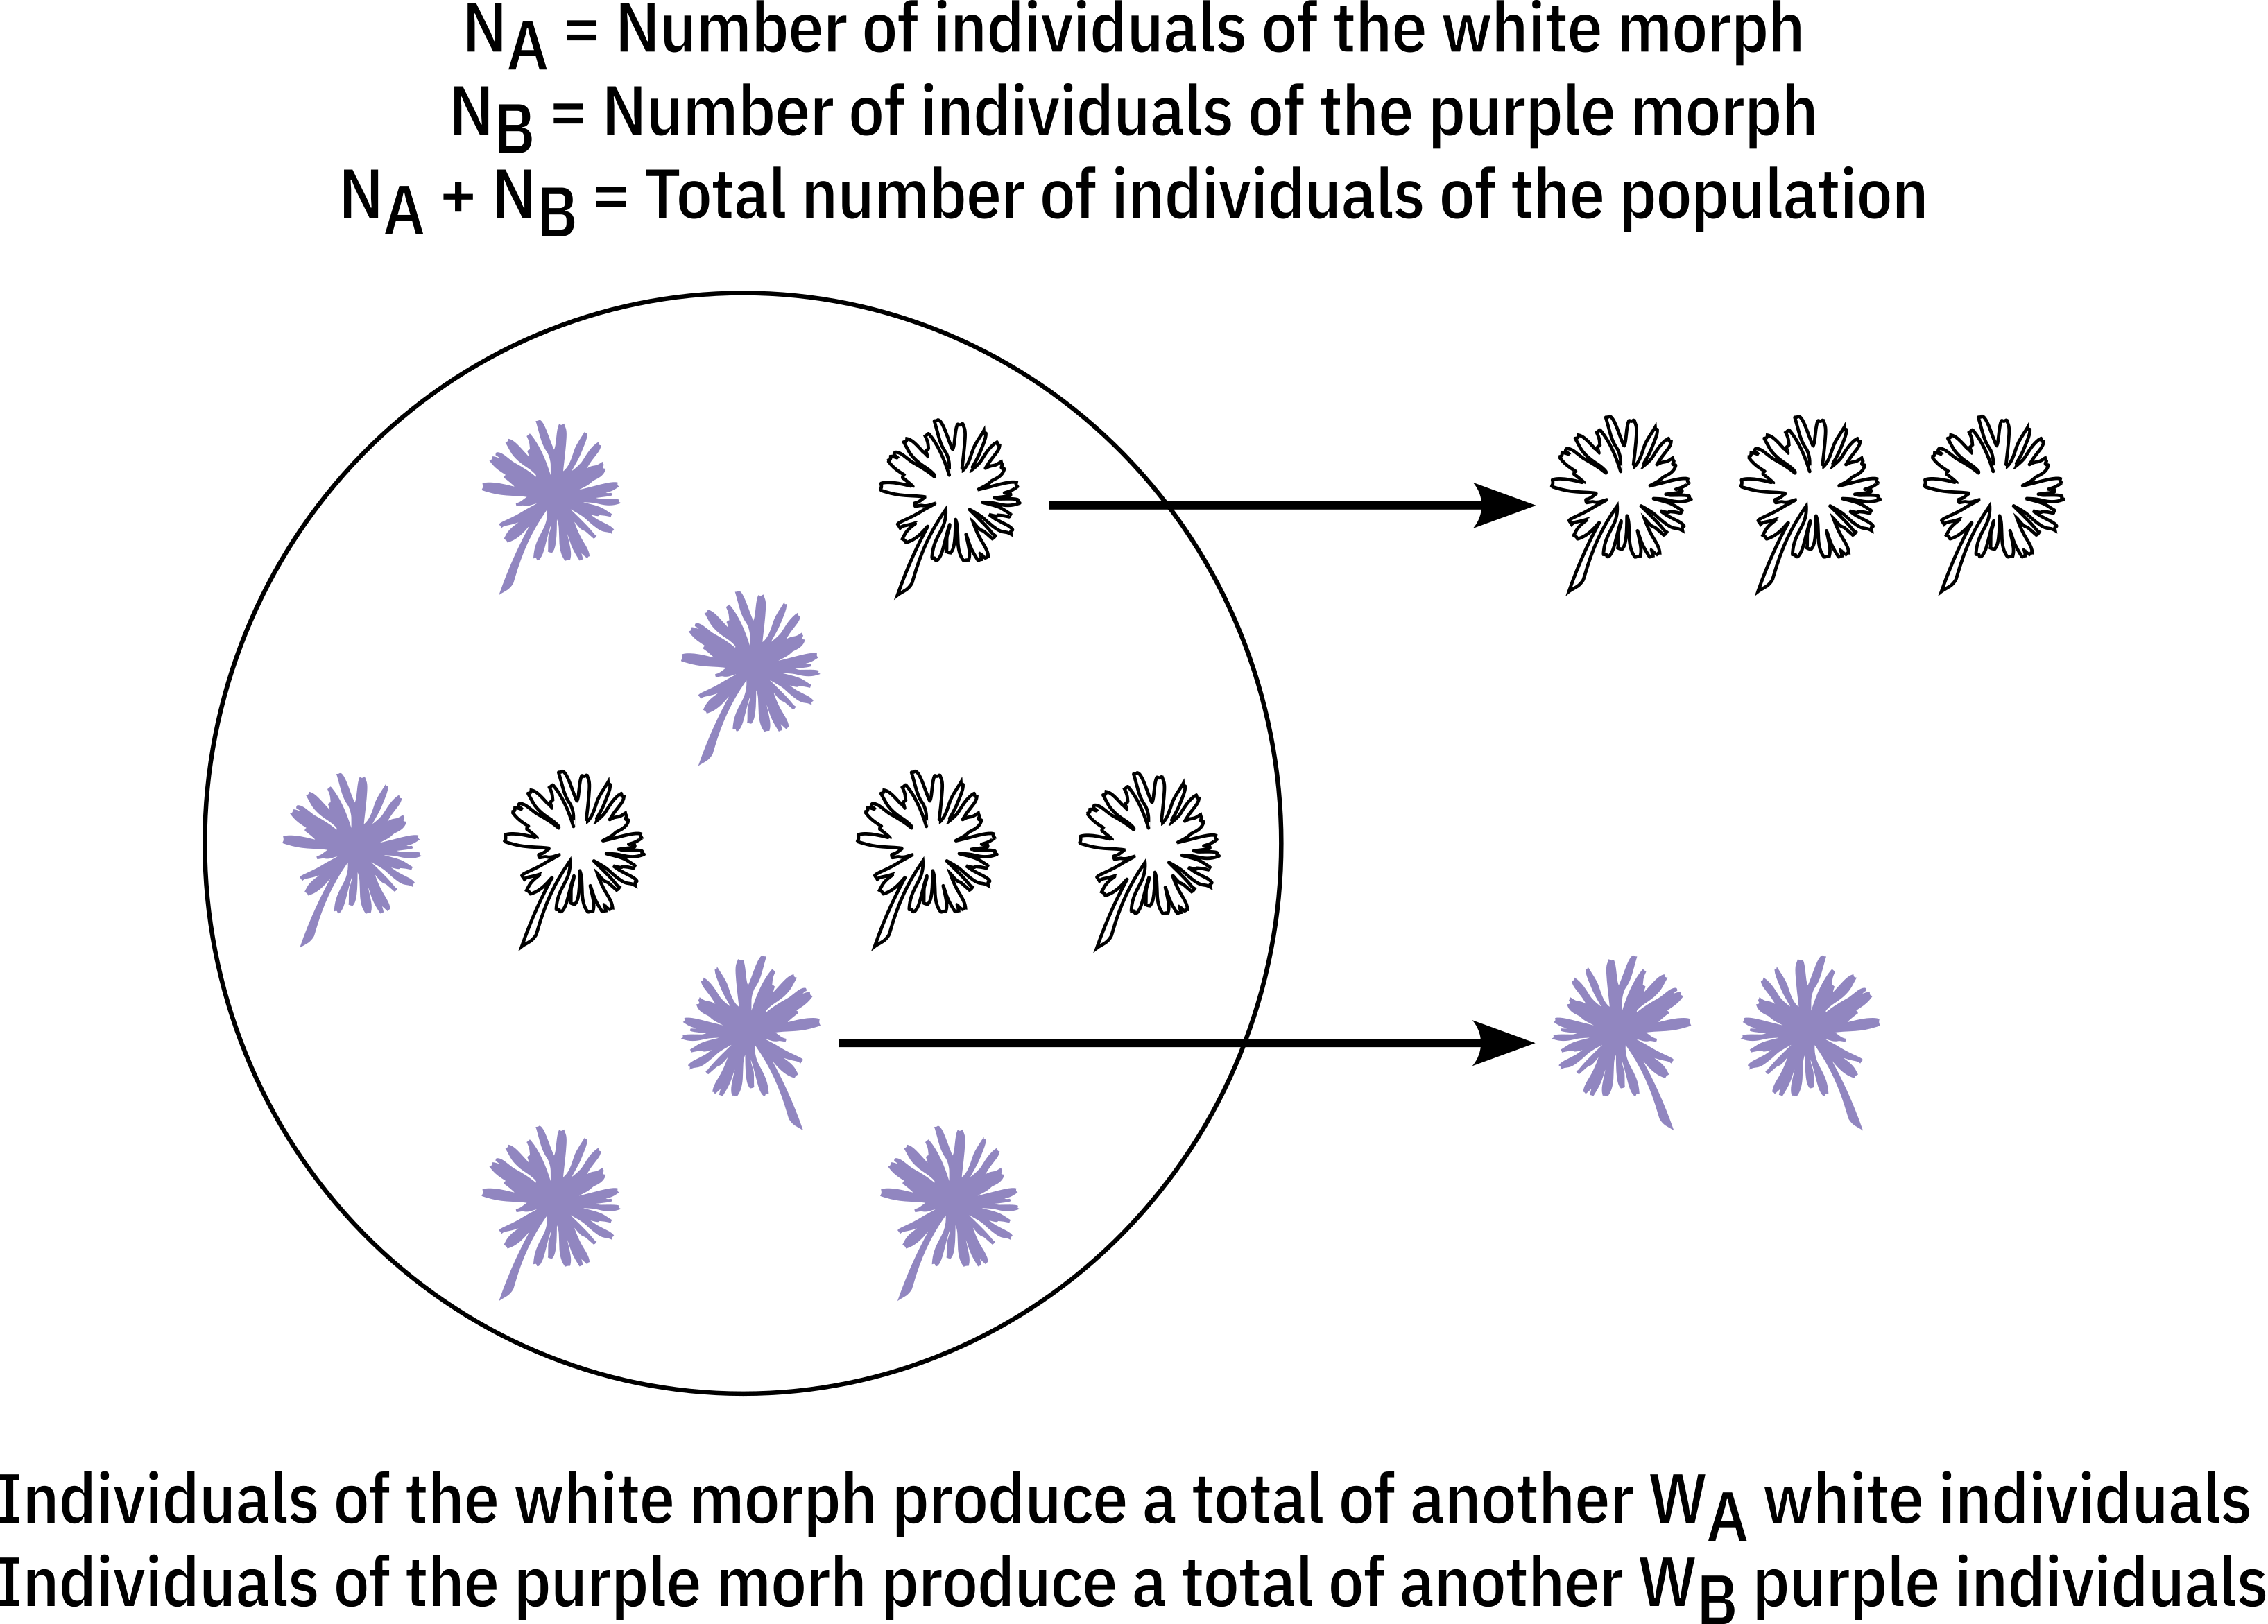
\includegraphics[width=0.65\textwidth,height=\textheight]{figs/fig1.png}
\caption{Fig. 1 - Theoretical example showing how the number of individuals of different morphs in a population can change from one generation to the other. For simplicity, in this example we assume that individuals are haploid and that two alleles, A and B, determine the white and purple floral morphs, respectively.}
\end{figure}

\(\\\)

Under the above assumptions, in the next generation the total number of individuals carrying the allele \(A\) in the population will depend on how much each individual contribute with offspring to the next generation. Mathematically, this is equivalent to multiply the current number of individuals carrying the allele \(A\), with their \emph{fitness}, as follows:

\[N_{A}^{(t+1)}=N_{A}^{(t)}W_{A}^{(t)}\]

where the superscripts \((t)\) and \((t+1)\) denotes the current and the next generation, respectively. Similarly, the following equation describes the number of individuals carrying the \(B\) allele in the next generation: \[N_{B}^{(t+1)}=N_{B}^{(t)}W_{B}^{(t)}\] However, we are interested in how the frequencies of these alleles change, not the absolute number of individuals. Since there are only two alleles in the population, if we find the frequency - \(p\) - of allele \(A\), then the frequency of \(B\) is equal to \((1-p)\). The frequency of \(A\) in the next generation is equal to the number of individuals carrying \(A\), divided by total number of individuals in the next generation, \(\frac{N_{A}^{(t+1)}}{N^{(t+1)}}\). We already know what \(N_{A}^{(t+1)}\) is, so our next step is to find what will be the total number of individuals in the next generation, \(N^{(t+1)}\). From the two equations above, we know that the total population size at the next generation is equal to:

\[N^{(t+1)}=N_{A}^{(t)}W_{A}^{(t)}+N_{B}^{(t)}W_{B}^{(t)}\]

We also know that at the current generation, the number of individuals carrying the allele \(A\), \(N_{A}^{(t)}\), is equal to the frequency of \(A\), multiplied by the total number of individuals in the population, that is \(N_{A}^{(t)}=p^{(t)}N^{(t)}\). In a similar way, \(N_{B}^{(t)}=(1-p^{(t)})N^{(t)}\). If we plug in these equivalences in the equation above, we get to the following one:

\[
\begin{aligned}
N^{(t+1)}&=N_{A}^{(t)}W_{A}^{(t)}+N_{B}^{(t)}W_{B}^{(t)} \\
N^{(t+1)}&=p^{(t)}N^{(t)}W_{A}^{(t)}+(1-p^{(t)})N^{(t)}W_{B}^{(t)}
\end{aligned}
\]

Further putting the \(N^{(t)}\) that appears at the right-hand side in evidence leads to:

\[
\begin{aligned}
N^{(t+1)}&=p^{(t)}N^{(t)}W_{A}^{(t)}+(1-p^{(t)})N^{(t)}W_{B}^{(t)} \\
N^{(t+1)}&=N^{(t)}\left[p^{(t)}W_{A}^{(t)}+(1-p^{(t)})W_{B}^{(t)} \right] \\
N^{(t+1)}&=N^{(t)}\overline{W}^{(t)}
\end{aligned}
\] where \(\overline{W}^{(t)}=p^{(t)}W_{A}^{(t)}+(1-p^{(t)})W_{B}^{(t)}\) is the average fitness of the population.

\[\begin{aligned}
\frac{N_{A}^{(t+1)}}{N^{(t+1)}}&=\frac{N_{A}^{(t)}W_{A}^{(t)}}{N^{(t)}\overline{W}^{(t)}} \\
p^{(t+1)}&=\frac{p^{(t)}W_{A}^{(t)}}{\overline{W}^{(t)}}
\end{aligned}\]

Now, lets try to understand what the equation above is telling us: at the next generation, the frequency of the allele \(A\) in the population will depend on the current frequency of \(A\), multiplied by the fraction \(\frac{W_{A}^{(t)}}{\overline{W}^{(t)}}\). This fraction represents the fitness of \(A\) relative to the average fitness in the population. On the one hand, if the fitness of \(A\) is larger than the average of the population, the fraction is higher than 1, and the frequency of \(A\) will increase in the next generation. On the other hand, when \(W_{A}^{(t)} < \overline{W}^{(t)}\), the fraction will be smaller than 1 and the frequency of \(A\) will decrease. What the equation is describing makes complete sense. If individuals of \(A\) reproduce more than the average, then, the frequency of \(A\) increases. This is exactly the way that we expect natural selection to operate, but now, we are able to \emph{quantify} this expected outcome.

\hypertarget{wrights-equation-for-the-adaptive-landscape-of-alleles}{%
\subsection{Wright's equation for the adaptive landscape of alleles}\label{wrights-equation-for-the-adaptive-landscape-of-alleles}}

We can gain further insight about how selection drive the frequencies of alleles if we come up with an expression for the \emph{change} in the frequency over generations, instead of just the frequency at the next generation. Mathematically, this is described by the difference \(p^{(t+1)} - p^{(t)}\), or \(\Delta p\) . Plugging in the expression for \(p^{(t+1)}\) that we just derived leads to the following equation:

\[\begin{aligned}
\Delta p&=p^{(t+1)} - p^{(t)} \\
\Delta p&=\frac{p^{(t)}W_{A}^{(t)}}{\overline{W}^{(t)}} - p^{(t)} \\
\Delta p&=\frac{p^{(t)}W_{A}^{(t)}}{\overline{W}^{(t)}} - \frac{p^{(t)}\overline{W}^{(t)}}{\overline{W}^{(t)}} \\
\Delta p&=p^{(t)}\frac{\left(W_{A}^{(t)}-\overline{W}^{(t)}\right)}{\overline{W}^{(t)}}
\end{aligned}\]

Substituting \(\overline{W}^{(t)}\) in the numerator with \(p^{(t)}W_{A}^{(t)}+(1-p^{(t)})W_{B}^{(t)}\) leads to:

\[\begin{aligned}
\Delta p&=p^{(t)}\frac{\left[W_{A}^{(t)}-p^{(t)}W_{A}^{(t)}-(1-p^{(t)})W_{B}^{(t)}\right]}{\overline{W}^{(t)}} \\
\Delta p&=p^{(t)}\frac{\left[(1-p^{(t)})W_{A}^{(t)}-(1-p^{(t)})W_{B}^{(t)}\right]}{\overline{W}^{(t)}} \\
\Delta p&=p^{(t)}(1-p^{(t)})\frac{\left(W_{A}^{(t)}-W_{B}^{(t)}\right)}{\overline{W}^{(t)}}
\end{aligned}\]

This equation show that the change in the frequency of the \(A\) allele depends on two components. First, it depends on \(p^{(t)}(1-p^{(t)})\). This term is the product of the frequencies of \(A\) and \(B\), which, from probability theory, represents the variance in frequencies. From this interpretation, the term \(p^{(t)}(1-p^{(t)})\) is the amount of genetic variance within the population. Second, the change in frequency also depends on the term \(\frac{\left(W_{A}-W_{B}^{(t)}\right)}{\overline{W}^{(t)}}\), representing the difference in fitness between individuals carrying the \(A\) or \(B\) alleles. When \(W_{A}>W_{B}\), this term is positive and it is negative when \(W_{A}<W_{B}\). Therefore, the equation shows that selection drives evolutionary changes depending on the amount of the available genetic variance within the population and differences in fitness. On the one hand genetic variance scales the amount of evolutionary change that can occur, such that if there is no genetic variance, i.e., \(p\neq 1\) and \(p\neq 0\), no change occurs. On the other hand, differences in fitness control the direction of the evolutionary changes. Since the variance is always a positive number, when \(W_{A}>W_{B}\), \(\Delta p\) is also positive and the frequency of \(p\) increases. In contrast, when \(W_{A}<W_{B}\), \(\Delta p\) will be negative and the frequency of \(p\) decreases. If there are no differences in fitness, or \(W_{A} = W_{B}\), there is no evolutionary change. Once more, this behavior makes complete sense from what we would expect from evolution by natural selection.

The equation above for the change in allele frequencies was the one derived by Sewall Wright in 1937 in the classic paper \emph{The distribution of gene frequencies in populations}. The key idea of the paper was identifying that the term \(\left(W_{A}^{(t)}-W_{B}^{(t)}\right)\) corresponds to the derivative of the average fitness of the population, relative to the frequency of allele \(p\), as follows:

\[\begin{aligned}
\frac{\partial \overline{W}^{(t)}}{\partial p} &= \frac{\partial}{\partial p^{(t)}}p^{(t)}W_{A}^{(t)} + \frac{\partial}{\partial p^{(t)}}(1-p^{(t)})W_{B}^{(t)} \\
\frac{\partial \overline{W}^{(t)}}{\partial p^{(t)}} &=  W_{A}^{(t)} - W_{B}^{(t)}
\end{aligned}\]

This result holds whenever the \emph{fitness} of alleles does not depend on their frequencies, or, in other words, when \emph{fitness} is frequency independent. The result above allow us to rewrite the equation for the change in allele frequencies as follows:

\[
\Delta p=p^{(t)}(1-p^{(t)})\frac{\partial ln\overline{W}^{(t)}}{\partial p^{(t)}}
\] where the \emph{ln} term in \(\frac{\partial ln\overline{W}^{(t)}}{\partial p^{(t)}}\) comes from the calculus rule that \(\frac{1}{x}\frac{d}{dx} = \frac{dlnx}{dx}\).

Rewriting the equation in terms of this derivative is key to understand the concept of how natural selection drive adaptations in populations. A derivative represents the slope of a curve at a point. In turn, the average \emph{fitness} of a population represents its growth rate. Thus, we can think about the derivative of the average fitness relative to the frequency of an allele as a population ``climbing'' a slope that is defined by the growth rate of the population. Visually this can be represented with the relationship between the average fitness of the population and the frequency of a given allele, as the figure below shows:

\begin{figure}
\centering
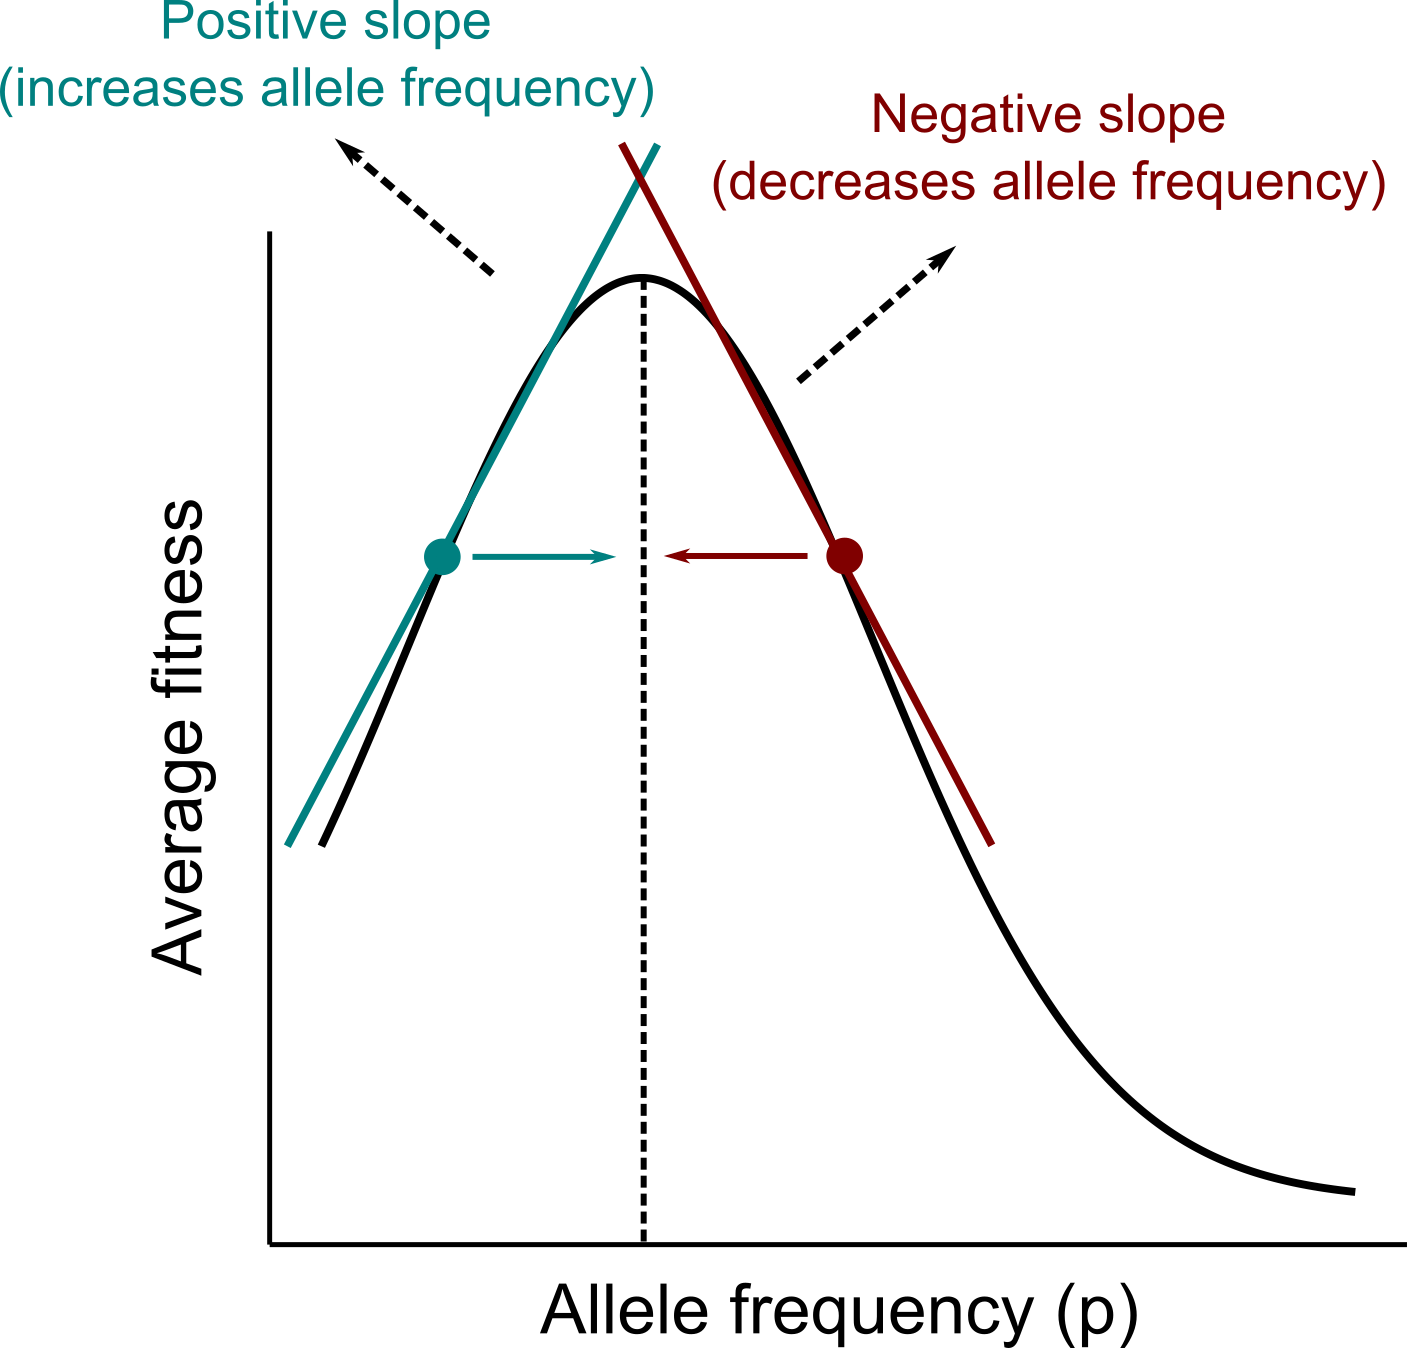
\includegraphics[width=0.5\textwidth,height=\textheight]{figs/fig2.png}
\caption{Fig. 2 - Hypothetical example of the relationship between the average fitness of a population and the frequency of an allele (p). The dashed line represents the point at which the slope (the derivative) is equal to 0. In the points to the left of the dashed line, the slope is positive, and selection favors an increase in the frequency of the allele. In contrast, the slope is negative in the points to the right of the dashed line and selection favors a decrease in the frequency of the allele. Importantly, across all points selection will drive the frequencies of the allele in the direction at which the average fitness of the population increases.}
\end{figure}

\(\\\)

The figure above illustrates the concept introduced by Wright (1937) of an \emph{adaptive landscape}. In evolutionary biology, the \emph{adaptive landscape} depicts the relationship between the average fitness of a population and the values of traits, which, in our example, are the frequencies of alleles. From the figure and the interpretation of the derivative outlined above, we can see the natural selection will drive the evolution of allele frequencies in the direction that increases the average fitness of the population. This provides a mathematical formulation and proof of the intuitive concept of how natural selection favors \emph{adaptations} in populations. This relationship always holds whenever \emph{fitness} is frequency-independent, but not when \emph{fitness} is frequency-dependent as we will see next in the exercise session.

Going back to our initial question: \textbf{how natural selection can drive changes in discrete or continuous traits in populations from one generation to the other?} Using Wright's equation we now can partially answer this question. For discrete traits, for instance, alleles, we learned that selection will favor the evolution of an increased frequency of alleles that maximize the average \emph{fitness} of the population, leading to \emph{adaptations}. The rate at which the population evolves will depend on the available genetic variation in the population, as well as how large are the differences in \emph{fitness} between individuals carrying different alleles.

\hypertarget{references}{%
\subsection{References}\label{references}}

Darwin, Charles Robert. 1861. \emph{On the Origin of Species by Means of Natural Selection, or the Preservation of Favoured Races in the Struggle for Life}. 3d edition. London: John Murray.

Futuyma, Douglas. 2005. \emph{Evolution}. Sunderland, MA: Sinauer Associates.

Levins, R. 1966. The strategy of model building in population biology. American Scientist 54 (4): 421--31.

Rice, Sean H. 2004. \emph{Evolutionary Theory: Mathematical and Conceptual Foundations}. New York, NY: Oxford University Press.

Turner, Derek and Joyce C. Havstad. 2019. Philosophy of Macroevolution. \emph{The Stanford Encyclopedia of Philosophy} (Summer 2019 Edition), Edward N. Zalta~(ed.). Available in: \url{https://plato.stanford.edu/archives/sum2019/entries/macroevolution}.

Wright, S. 1937. The distribution of gene frequencies in populations. \emph{Proceedings of the National Academy of Sciences of the United States of America} 23 (6): 307--20.

\hypertarget{exercise-evolution-of-allele-frequencies}{%
\chapter{Exercise: Evolution of allele frequencies}\label{exercise-evolution-of-allele-frequencies}}

\hypertarget{simulating-evolutionary-changes-in-allele-frequencies}{%
\section{Simulating evolutionary changes in allele frequencies}\label{simulating-evolutionary-changes-in-allele-frequencies}}

In the first lecture we studied and derived the classical Wright's equation that predicts how natural selection can drive changes in the frequency of alleles over generations in a population. Throughout this exercise section, we will perform numerical simulations of this equation to gain more intuition about how evolution will proceed under different scenarios. We begin with the equation that we are trying to simulate:

\[
\Delta p=p^{(t)}(1-p^{(t)})\frac{\left(W_{A}^{(t)}-W_{B}^{(t)}\right)}{\overline{W}^{(t)}}
\]

Our first step is to define a vector that will store the frequencies, \(p\) at each time step (generation) of the model, and an initial frequency of \(p\), \(p_{0}\). The choice of initial value is arbitrary and depends on your particular problem. Here we will start with \(p_{0}=0.1\), but feel free to use and explore different values.

\begin{Shaded}
\begin{Highlighting}[]
\NormalTok{dp }\OtherTok{=} \FunctionTok{c}\NormalTok{()}
\NormalTok{p0 }\OtherTok{=} \FloatTok{0.1}
\NormalTok{dp[}\DecValTok{1}\NormalTok{] }\OtherTok{=}\NormalTok{ p0}
\end{Highlighting}
\end{Shaded}

Now, we need to code how \(p\) gets updated at each time step. From the equation, \(p\) gets updated depending on its value at the current time step, \(t\), and the \emph{fitness} of individuals carrying the alleles \(A\) or \(B\). So, we also need to define what are the fitness functions of these individuals. We will explore different scenarios, but we will begin with a constant value:

\begin{Shaded}
\begin{Highlighting}[]
\NormalTok{wA }\OtherTok{=} \DecValTok{2}
\NormalTok{wB }\OtherTok{=} \DecValTok{1}
\end{Highlighting}
\end{Shaded}

Now, we need to iterate over the equation so that we can obtain the frequencies at future generations. To do so, we will first define for how many generations, \(t_{max}\), we will run the simulation. Then, we will use a \emph{for loop} to perform the iterations. In the \emph{for loop} we will go through the following steps:

\begin{enumerate}
\def\labelenumi{\arabic{enumi}.}
\item
  Set the value of \(p\) to the one at the current time step, \(t\)
\item
  Compute the average fitness of the population as \(pW_{A}+(1-p)W_{B}\)
\item
  Update the value of \(p\) using Wright's equation
\end{enumerate}

These steps are highlighted in the block of code below:

\begin{Shaded}
\begin{Highlighting}[]
\NormalTok{tmax }\OtherTok{=} \DecValTok{50} \CommentTok{\# The simulation will run for 50 generations}

\ControlFlowTok{for}\NormalTok{(t }\ControlFlowTok{in} \DecValTok{1}\SpecialCharTok{:}\NormalTok{(tmax}\DecValTok{{-}1}\NormalTok{))\{ }\CommentTok{\#Setting up the for loop}
  
\NormalTok{  p }\OtherTok{=}\NormalTok{ dp[t] }\CommentTok{\# Step 1}
\NormalTok{  w\_avg }\OtherTok{=}\NormalTok{ p}\SpecialCharTok{*}\NormalTok{wA }\SpecialCharTok{+}\NormalTok{ (}\DecValTok{1}\SpecialCharTok{{-}}\NormalTok{p)}\SpecialCharTok{*}\NormalTok{wB }\CommentTok{\#Step 2}
\NormalTok{  dp[t}\SpecialCharTok{+}\DecValTok{1}\NormalTok{]}\OtherTok{=}\NormalTok{ p }\SpecialCharTok{+}\NormalTok{ (p}\SpecialCharTok{*}\NormalTok{(}\DecValTok{1}\SpecialCharTok{{-}}\NormalTok{p)}\SpecialCharTok{*}\NormalTok{(wA}\SpecialCharTok{{-}}\NormalTok{wB)}\SpecialCharTok{/}\NormalTok{w\_avg) }\CommentTok{\#Step 3}
\NormalTok{\}}
\end{Highlighting}
\end{Shaded}

That is it! We have performed our first numerical simulation. Now that we have the outcome along generations, we can plot the results. To plot the results, we first set up a data frame with columns containing the outcome on our variable of interest. This variable is called a \emph{state variable} and here it is the frequency of \(p\) over the 50 generations of the population. With the data frame set up, we can plot how the \emph{state variable} (on the y-axis) changes over the generations (x-axis). You can use a plot method of your choice. Here we are going to use the package \emph{ggplot2} for all of the plots. The code to perform the steps above can be found below:

\begin{Shaded}
\begin{Highlighting}[]
\FunctionTok{library}\NormalTok{(ggplot2)}
\FunctionTok{library}\NormalTok{(ggpubr)}

\NormalTok{r }\OtherTok{=} \FunctionTok{data.frame}\NormalTok{(}\AttributeTok{dp=}\NormalTok{dp, }\AttributeTok{t=}\DecValTok{1}\SpecialCharTok{:}\NormalTok{tmax)}

\FunctionTok{ggplot}\NormalTok{()}\SpecialCharTok{+}
  \FunctionTok{geom\_line}\NormalTok{(}\AttributeTok{data=}\NormalTok{r, }\FunctionTok{aes}\NormalTok{(}\AttributeTok{x=}\NormalTok{t, }\AttributeTok{y=}\NormalTok{dp))}\SpecialCharTok{+}
  \FunctionTok{xlab}\NormalTok{(}\StringTok{"Generation"}\NormalTok{)}\SpecialCharTok{+}\FunctionTok{ylab}\NormalTok{(}\StringTok{"Frequency of allele A"}\NormalTok{)}\SpecialCharTok{+}
  \FunctionTok{theme\_pubr}\NormalTok{()}
\end{Highlighting}
\end{Shaded}

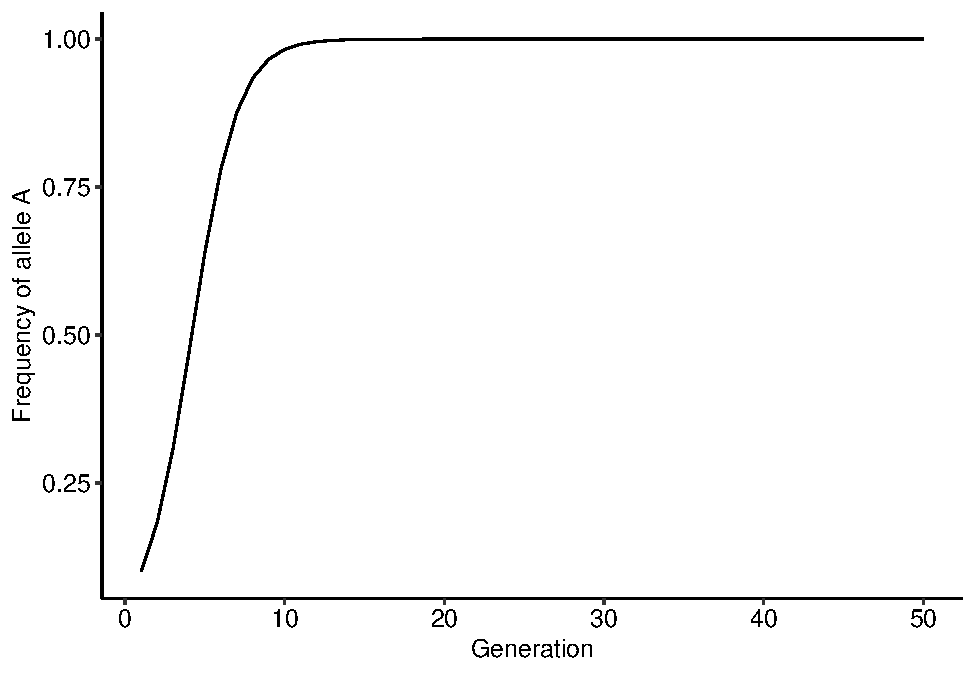
\includegraphics[width=0.65\linewidth,height=0.65\textheight]{_main_files/figure-latex/unnamed-chunk-4-1}

Now that we have the code to perform the numerical simulations, it is convenient to put everything inside a function. For this example, our function will take as input arguments \(t_{max}\), \(W_{A}\), \(W_{B}\) and the initial frequency of allele A in the population, \(p_{0}\). Then, the function will run the simulation and return a data frame containing the different values of \(p\) over the \(t_{max}\) generations of the simulation. The code of the implement the function is as follows:

\begin{Shaded}
\begin{Highlighting}[]
\NormalTok{evo\_simulation}\OtherTok{\textless{}{-}}\ControlFlowTok{function}\NormalTok{(tmax, p0, wA, wB)\{ }\CommentTok{\#Defining the function and the input arguments}
  
\NormalTok{  dp }\OtherTok{=} \FunctionTok{c}\NormalTok{() }\CommentTok{\#Creating the vector to store the outcome}
\NormalTok{  dp[}\DecValTok{1}\NormalTok{]}\OtherTok{\textless{}{-}}\NormalTok{p0 }\CommentTok{\#Setting the initial frequency of p}
  
  \ControlFlowTok{for}\NormalTok{(t }\ControlFlowTok{in} \DecValTok{1}\SpecialCharTok{:}\NormalTok{(tmax}\DecValTok{{-}1}\NormalTok{))\{ }\CommentTok{\#Setting up the for loop}
  
\NormalTok{  p }\OtherTok{=}\NormalTok{ dp[t] }\CommentTok{\# Step 1}
\NormalTok{  w\_avg }\OtherTok{=}\NormalTok{ p}\SpecialCharTok{*}\NormalTok{wA }\SpecialCharTok{+}\NormalTok{ (}\DecValTok{1}\SpecialCharTok{{-}}\NormalTok{p)}\SpecialCharTok{*}\NormalTok{wB }\CommentTok{\#Step 2}
\NormalTok{  dp[t}\SpecialCharTok{+}\DecValTok{1}\NormalTok{]}\OtherTok{=}\NormalTok{ p }\SpecialCharTok{+}\NormalTok{ (p}\SpecialCharTok{*}\NormalTok{(}\DecValTok{1}\SpecialCharTok{{-}}\NormalTok{p)}\SpecialCharTok{*}\NormalTok{(wA}\SpecialCharTok{{-}}\NormalTok{wB)}\SpecialCharTok{/}\NormalTok{w\_avg) }\CommentTok{\#Step 3}
\NormalTok{\}}
  
\NormalTok{  r }\OtherTok{=} \FunctionTok{data.frame}\NormalTok{(}\AttributeTok{dp=}\NormalTok{dp, }\AttributeTok{t=}\DecValTok{1}\SpecialCharTok{:}\NormalTok{tmax) }\CommentTok{\# Building the data frame}
  
  \FunctionTok{return}\NormalTok{(r)}
  
\NormalTok{\}}

\CommentTok{\# Running the function to test it:}

\NormalTok{r }\OtherTok{=} \FunctionTok{evo\_simulation}\NormalTok{(}\AttributeTok{tmax=}\DecValTok{50}\NormalTok{, }\AttributeTok{p0=}\FloatTok{0.2}\NormalTok{, }\AttributeTok{wA=}\DecValTok{2}\NormalTok{, }\AttributeTok{wB=}\DecValTok{1}\NormalTok{)}

\CommentTok{\# Plotting the result}

\FunctionTok{ggplot}\NormalTok{()}\SpecialCharTok{+}
  \FunctionTok{geom\_line}\NormalTok{(}\AttributeTok{data=}\NormalTok{r, }\FunctionTok{aes}\NormalTok{(}\AttributeTok{x=}\NormalTok{t, }\AttributeTok{y=}\NormalTok{dp))}\SpecialCharTok{+}
  \FunctionTok{xlab}\NormalTok{(}\StringTok{"Generation"}\NormalTok{)}\SpecialCharTok{+}\FunctionTok{ylab}\NormalTok{(}\StringTok{"Frequency of allele A"}\NormalTok{)}\SpecialCharTok{+}
  \FunctionTok{theme\_pubr}\NormalTok{()}
\end{Highlighting}
\end{Shaded}

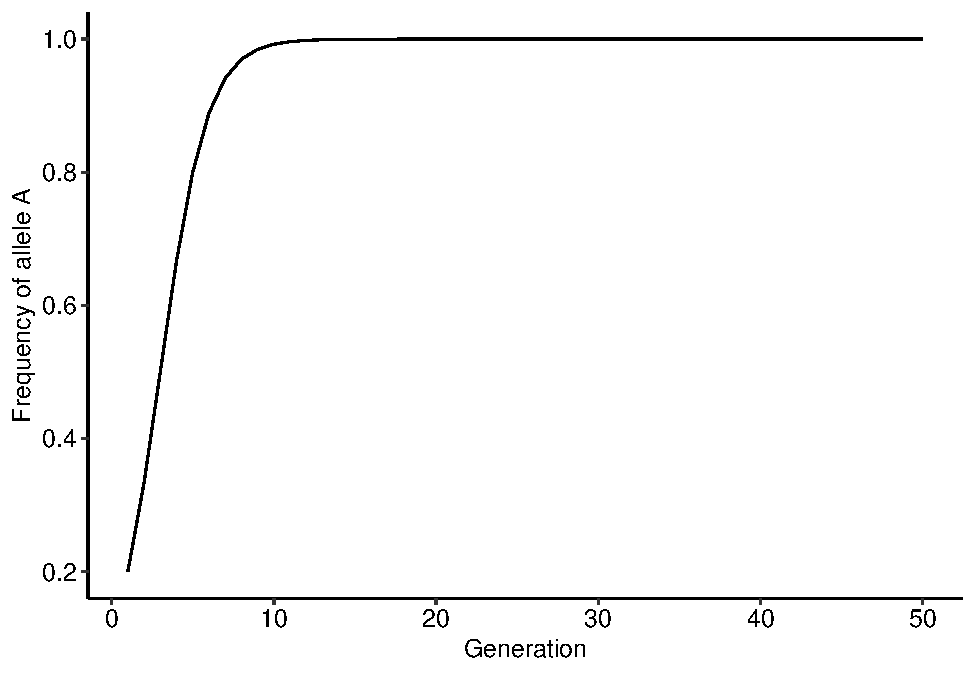
\includegraphics[width=0.65\linewidth,height=0.65\textheight]{_main_files/figure-latex/unnamed-chunk-5-1}

Now that we have a function that makes it very easy to simulate the changes in allele frequencies, try to explore how different values of \(p_{0}\), \(W_{A}\) and \(W_{B}\) affect the evolutionary dynamics. Try to also explore how different values of \(t_{max}\), or the time scale that we are looking at, can change our perception about how evolution is unfolding in a population.

\hypertarget{using-different-assumptions-for-the-fitness-of-alleles-a-and-b}{%
\section{Using different assumptions for the fitness of alleles A and B}\label{using-different-assumptions-for-the-fitness-of-alleles-a-and-b}}

In the previous section we simulated the evolutionary dynamics of allele frequencies when the fitness of individuals carrying either one of the alleles are constant values. However, what would happen when fitness can change over time? Now, we will explore the evolutionary dynamics when \(W_{A}\) and \(W_{B}\) depends not only on constant value but also can vary with the frequency of allele \(A\) or \(B\). This is the case mentioned in the lecture notes that correspond to frequency-dependent values of fitness. To understand how frequency-dependence can affect the outcome, we will assume that \(W_{A}\) and \(W_{B}\) have the same constant baseline value, but can decrease with the frequency of their corresponding allele. This can be represented with the following two equations:

\[\begin{align}
W_{A}^{(t)}&=1-\alpha p^{(t)} \\
W_{B}^{(t)}&=1-\beta (1-p^{(t)})
\end{align}\]

where \(\alpha\) and \(\beta\) weight how much \(W_{A}\) and \(W_{B}\) is decreased depending on the frequency of alleles \(A\) and \(B\), respectively. Since it does not make biological sense to have negative fitness values, we just need to choose the values of \(\alpha\) and \(\beta\) so that fitness is never negative. Under this assumption, we can now build a now function that take as input arguments the \emph{parameters} \(\alpha\) and \(\beta\), instead of the constant values of \(W_{A}\) and \(W_{B}\). The difference is that because fitness can vary across time, at each time step of the model we need to recompute fitness values. The code for the modified function is depicted below:

\begin{Shaded}
\begin{Highlighting}[]
\NormalTok{evo\_simulation}\OtherTok{\textless{}{-}}\ControlFlowTok{function}\NormalTok{(tmax, p0, alpha, beta)\{ }\CommentTok{\#Defining the function and the input arguments}
  
\NormalTok{  dp }\OtherTok{=} \FunctionTok{c}\NormalTok{() }\CommentTok{\#Creating the vector to store the outcome}
\NormalTok{  dp[}\DecValTok{1}\NormalTok{]}\OtherTok{\textless{}{-}}\NormalTok{p0 }\CommentTok{\#Setting the initial frequency of p}
  
  \ControlFlowTok{for}\NormalTok{(t }\ControlFlowTok{in} \DecValTok{1}\SpecialCharTok{:}\NormalTok{(tmax}\DecValTok{{-}1}\NormalTok{))\{ }\CommentTok{\#Setting up the for loop}
  
\NormalTok{  p }\OtherTok{=}\NormalTok{ dp[t] }\CommentTok{\# Setting current frequency}
\NormalTok{  wA }\OtherTok{=} \DecValTok{1}\SpecialCharTok{{-}}\NormalTok{(alpha}\SpecialCharTok{*}\NormalTok{p) }\CommentTok{\#Computing the fitness of A at the current generation}
\NormalTok{  wB }\OtherTok{=} \DecValTok{1}\SpecialCharTok{{-}}\NormalTok{(beta}\SpecialCharTok{*}\NormalTok{(}\DecValTok{1}\SpecialCharTok{{-}}\NormalTok{p)) }\CommentTok{\#Computing the fitness of B at the current generation}
\NormalTok{  w\_avg }\OtherTok{=}\NormalTok{ p}\SpecialCharTok{*}\NormalTok{wA }\SpecialCharTok{+}\NormalTok{ (}\DecValTok{1}\SpecialCharTok{{-}}\NormalTok{p)}\SpecialCharTok{*}\NormalTok{wB }\CommentTok{\#Computing the average fitness of the population}
\NormalTok{  dp[t}\SpecialCharTok{+}\DecValTok{1}\NormalTok{]}\OtherTok{=}\NormalTok{ p }\SpecialCharTok{+}\NormalTok{ (p}\SpecialCharTok{*}\NormalTok{(}\DecValTok{1}\SpecialCharTok{{-}}\NormalTok{p)}\SpecialCharTok{*}\NormalTok{(wA}\SpecialCharTok{{-}}\NormalTok{wB)}\SpecialCharTok{/}\NormalTok{w\_avg) }\CommentTok{\#Updating frequencies}
\NormalTok{\}}
  
\NormalTok{  r }\OtherTok{=} \FunctionTok{data.frame}\NormalTok{(}\AttributeTok{dp=}\NormalTok{dp, }\AttributeTok{t=}\DecValTok{1}\SpecialCharTok{:}\NormalTok{tmax) }\CommentTok{\# Building the data frame}
  
  \FunctionTok{return}\NormalTok{(r)}
  
\NormalTok{\}}

\CommentTok{\# Running the function to test it:}

\NormalTok{r }\OtherTok{=} \FunctionTok{evo\_simulation}\NormalTok{(}\AttributeTok{tmax=}\DecValTok{50}\NormalTok{, }\AttributeTok{p0=}\FloatTok{0.2}\NormalTok{, }\AttributeTok{alpha=}\FloatTok{0.1}\NormalTok{, }\AttributeTok{beta=}\FloatTok{0.2}\NormalTok{)}

\CommentTok{\# Plotting the result}

\FunctionTok{ggplot}\NormalTok{()}\SpecialCharTok{+}
  \FunctionTok{geom\_line}\NormalTok{(}\AttributeTok{data=}\NormalTok{r, }\FunctionTok{aes}\NormalTok{(}\AttributeTok{x=}\NormalTok{t, }\AttributeTok{y=}\NormalTok{dp))}\SpecialCharTok{+}
  \FunctionTok{xlab}\NormalTok{(}\StringTok{"Generation"}\NormalTok{)}\SpecialCharTok{+}\FunctionTok{ylab}\NormalTok{(}\StringTok{"Frequency of allele A"}\NormalTok{)}\SpecialCharTok{+}
  \FunctionTok{scale\_y\_continuous}\NormalTok{(}\AttributeTok{limits=}\FunctionTok{c}\NormalTok{(}\DecValTok{0}\NormalTok{,}\DecValTok{1}\NormalTok{))}\SpecialCharTok{+} \CommentTok{\#Setting the limits on the y{-}axis to be the same as in the previous model}
  \FunctionTok{theme\_pubr}\NormalTok{()}
\end{Highlighting}
\end{Shaded}

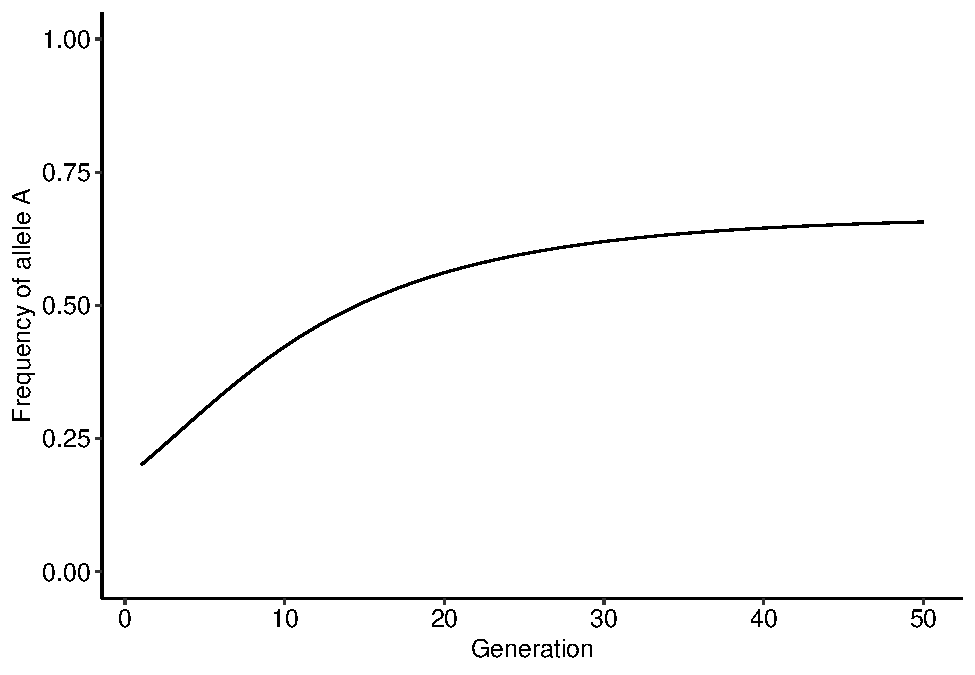
\includegraphics[width=0.65\linewidth,height=0.65\textheight]{_main_files/figure-latex/unnamed-chunk-6-1}

With this new function, explore how different values of \(\alpha\), \(\beta\) and \(p_{0}\) change the outcome. In your exploration, try to answer the following questions:

\begin{enumerate}
\def\labelenumi{\arabic{enumi}.}
\item
  How frequency-dependence changes the outcome of the evolutionary dynamics?
\item
  Does the initial value of allele frequency in the population affect the final outcome?
\item
  What is the role of \(\alpha\) and \(\beta\) in the outcome of the dynamics?
\item
  What would be an ecological mechanism that can lead to the type of frequency dependence that we are exploring? What ecological pattern would you expect under this mechanism over the generations of a population?
\end{enumerate}

\hypertarget{simulating-wrights-adaptive-landscape}{%
\section{Simulating Wright's adaptive landscape}\label{simulating-wrights-adaptive-landscape}}

Until now we have explored the evolutionary dynamics of allele frequencies a population under different assumptions of the fitness of individuals carrying these alleles. In the lecture notes we saw that the evolutionary dynamics of these alleles can be visualized as populations embedded in a fitness landscape, depicting the relationship between the average fitness of a population and trait values. We also studied that the direction and magnitude of the evolutionary change is given by the slope in this landscape at a particular point of allele frequency. Here, we will explore how we can visualize the fitness landscape of the populations and how the populations move across this landscape along the evolutionary dynamics. In our example, the fitness landscape depicts the relationship between the average fitness of the population and the frequency of one allele. Therefore, to build this landscape we need to simulate what would be the average fitness of a population for many different values of allele frequency. To do so, we will perform the following steps:

\begin{enumerate}
\def\labelenumi{\arabic{enumi}.}
\item
  Define the fitness of alleles \(A\) and \(B\)
\item
  Build a vector containing many different values of \(p\), varying from 0 to 1.
\item
  Compute the average fitness of the population, \(\overline{W}\), for each of these values of \(p\).
\item
  Plot and visualize the fitness landscape.
\end{enumerate}

We will begin with constant fitness values, and then, will explore how the landscape changes with frequency-dependent fitness values. These three steps are implemented and highlighted in the code below:

\begin{Shaded}
\begin{Highlighting}[]
\NormalTok{wA }\OtherTok{=} \DecValTok{2} \CommentTok{\# Step 1}
\NormalTok{wB }\OtherTok{=} \DecValTok{1} \CommentTok{\# Step 1}
\NormalTok{p }\OtherTok{=} \FunctionTok{seq}\NormalTok{(}\DecValTok{0}\NormalTok{, }\DecValTok{1}\NormalTok{, }\FloatTok{0.001}\NormalTok{) }\CommentTok{\# Step 2}
\NormalTok{w\_avg }\OtherTok{=}\NormalTok{ p}\SpecialCharTok{*}\NormalTok{wA }\SpecialCharTok{+}\NormalTok{ (}\DecValTok{1}\SpecialCharTok{{-}}\NormalTok{p)}\SpecialCharTok{*}\NormalTok{wB }\CommentTok{\#Step 3}

\NormalTok{land }\OtherTok{=} \FunctionTok{data.frame}\NormalTok{(p, w\_avg) }\CommentTok{\#Building a data frame with values of p and the corresponding average fitness}

\CommentTok{\# Plotting the landscape.}

\FunctionTok{ggplot}\NormalTok{()}\SpecialCharTok{+}
  \FunctionTok{geom\_line}\NormalTok{(}\AttributeTok{data=}\NormalTok{land, }\FunctionTok{aes}\NormalTok{(}\AttributeTok{x=}\NormalTok{p, }\AttributeTok{y=}\NormalTok{w\_avg))}\SpecialCharTok{+}
  \FunctionTok{xlab}\NormalTok{(}\StringTok{"Frequency of allele A"}\NormalTok{)}\SpecialCharTok{+}\FunctionTok{ylab}\NormalTok{(}\StringTok{"Average fitness of the population"}\NormalTok{)}\SpecialCharTok{+}
  \FunctionTok{theme\_pubr}\NormalTok{()}
\end{Highlighting}
\end{Shaded}

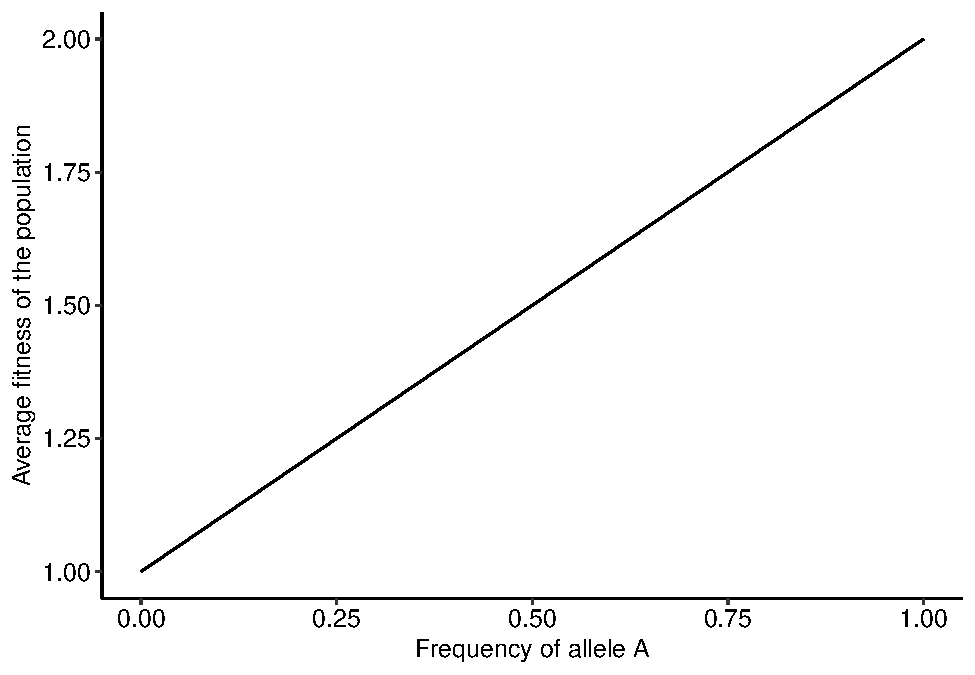
\includegraphics[width=0.65\linewidth,height=0.65\textheight]{_main_files/figure-latex/unnamed-chunk-7-1}

Well, this landscape resembles much more a ``ladder'' than a proper landscape. However, this makes complete sense when we think about the relationship between \(\overline{W}\) and \(p\) when fitness are constant values. In fact, we can understand this relationship better with the equation for \(\overline{W}\) as a function of \(p\), as follows:

\[\begin{aligned}
\overline{W}^{(t)}&=p^{(t)}W_{A} + (1-p^{(t)})W_{B} \\
\overline{W}^{(t)}&=p^{(t)}W_{A} + W_{B} - p^{(t)}W_{B}
\overline{W}^{(t)}&=W_{B}+(W_{A}-W_{B})p^{(t)}
\end{aligned}\]

The equation above shows that the relationship between \(\overline{W}\) and \(p\) is the equation of a line. The line has intercept equal to \(W_{B}\) and slope equal to \((W_{A}-W_{B})\). It is this slope that will determine the direction of evolutionary change. Now that we know how to build the landscape under a fitness function, we can also visualize how populations move in this landscape. We first build the landscape. Then, we use our function to simulate the evolutionary dynamics and plot the position of our population in the landscape in different generations. It is easier if we put everything inside a single function as we can find below:

\begin{Shaded}
\begin{Highlighting}[]
\FunctionTok{library}\NormalTok{(viridis)}
\end{Highlighting}
\end{Shaded}

\begin{verbatim}
## Loading required package: viridisLite
\end{verbatim}

\begin{Shaded}
\begin{Highlighting}[]
\NormalTok{evo\_landscape}\OtherTok{\textless{}{-}}\ControlFlowTok{function}\NormalTok{(tmax, p0, wA, wB)\{ }\CommentTok{\#Defining the function and the input arguments}
  
\NormalTok{p\_theo }\OtherTok{=} \FunctionTok{seq}\NormalTok{(}\DecValTok{0}\NormalTok{, }\DecValTok{1}\NormalTok{, }\FloatTok{0.001}\NormalTok{) }\CommentTok{\# Defining the theoretical values of p to build the fitness landscape}
\NormalTok{w\_avg\_theo }\OtherTok{=}\NormalTok{ p\_theo}\SpecialCharTok{*}\NormalTok{wA }\SpecialCharTok{+}\NormalTok{ (}\DecValTok{1}\SpecialCharTok{{-}}\NormalTok{p\_theo)}\SpecialCharTok{*}\NormalTok{wB }\CommentTok{\#Computing the average fitness}
\NormalTok{land }\OtherTok{=} \FunctionTok{data.frame}\NormalTok{(p\_theo, w\_avg\_theo) }\CommentTok{\#Building a data frame with values of p and the corresponding average fitness}
  
\NormalTok{dp }\OtherTok{=} \FunctionTok{c}\NormalTok{() }\CommentTok{\#Creating the vector to store the outcome}
\NormalTok{dw }\OtherTok{=} \FunctionTok{c}\NormalTok{() }\CommentTok{\#Creating a vector to keep track of the average fitness along the evolutionary dynamics}
\NormalTok{dp[}\DecValTok{1}\NormalTok{]}\OtherTok{\textless{}{-}}\NormalTok{p0 }\CommentTok{\#Setting the initial frequency of p}
  
  \ControlFlowTok{for}\NormalTok{(t }\ControlFlowTok{in} \DecValTok{1}\SpecialCharTok{:}\NormalTok{(tmax}\DecValTok{{-}1}\NormalTok{))\{ }\CommentTok{\#Setting up the for loop}
  
\NormalTok{  p }\OtherTok{=}\NormalTok{ dp[t] }\CommentTok{\# Setting current frequencies}
\NormalTok{  w\_avg }\OtherTok{=}\NormalTok{ p}\SpecialCharTok{*}\NormalTok{wA }\SpecialCharTok{+}\NormalTok{ (}\DecValTok{1}\SpecialCharTok{{-}}\NormalTok{p)}\SpecialCharTok{*}\NormalTok{wB }\CommentTok{\# Computing average fitness}
\NormalTok{  dw[t] }\OtherTok{=}\NormalTok{ w\_avg}
\NormalTok{  dp[t}\SpecialCharTok{+}\DecValTok{1}\NormalTok{]}\OtherTok{=}\NormalTok{ p }\SpecialCharTok{+}\NormalTok{ (p}\SpecialCharTok{*}\NormalTok{(}\DecValTok{1}\SpecialCharTok{{-}}\NormalTok{p)}\SpecialCharTok{*}\NormalTok{(wA}\SpecialCharTok{{-}}\NormalTok{wB)}\SpecialCharTok{/}\NormalTok{w\_avg) }\CommentTok{\#Updating frequency values}
  
\NormalTok{\}}
\NormalTok{  dw[tmax] }\OtherTok{=}\NormalTok{  dp[tmax]}\SpecialCharTok{*}\NormalTok{wA }\SpecialCharTok{+}\NormalTok{ (}\DecValTok{1}\SpecialCharTok{{-}}\NormalTok{dp[tmax])}\SpecialCharTok{*}\NormalTok{wB }\CommentTok{\#Computing average fitness for the final time step}
\NormalTok{  r }\OtherTok{=} \FunctionTok{data.frame}\NormalTok{(}\AttributeTok{dp=}\NormalTok{dp, dw, }\AttributeTok{t=}\DecValTok{1}\SpecialCharTok{:}\NormalTok{tmax) }\CommentTok{\# Building the data frame}
  
  \FunctionTok{return}\NormalTok{(}\FunctionTok{list}\NormalTok{(land, r)) }\CommentTok{\# Returning a list with the data frame of the dynamics and the landscape, respectively}
  
\NormalTok{\}}
\CommentTok{\# Running the function to test it:}

\NormalTok{r\_list }\OtherTok{=} \FunctionTok{evo\_landscape}\NormalTok{(}\AttributeTok{tmax=}\DecValTok{20}\NormalTok{, }\AttributeTok{p0=}\FloatTok{0.2}\NormalTok{, }\AttributeTok{wA=}\FloatTok{1.5}\NormalTok{, }\AttributeTok{wB=}\DecValTok{1}\NormalTok{)}

\CommentTok{\# Plotting the landscape and how the population moves over generations}

\FunctionTok{ggplot}\NormalTok{()}\SpecialCharTok{+}
  \FunctionTok{geom\_line}\NormalTok{(}\AttributeTok{data=}\NormalTok{r\_list[[}\DecValTok{1}\NormalTok{]], }\FunctionTok{aes}\NormalTok{(}\AttributeTok{x=}\NormalTok{p\_theo, }\AttributeTok{y=}\NormalTok{w\_avg\_theo))}\SpecialCharTok{+}
  \FunctionTok{geom\_point}\NormalTok{(}\AttributeTok{data=}\NormalTok{r\_list[[}\DecValTok{2}\NormalTok{]], }\FunctionTok{aes}\NormalTok{(}\AttributeTok{x=}\NormalTok{dp, }\AttributeTok{y=}\NormalTok{dw, }\AttributeTok{fill=}\NormalTok{t), }\AttributeTok{color=}\StringTok{"black"}\NormalTok{, }\AttributeTok{shape=}\DecValTok{21}\NormalTok{, }\AttributeTok{size=}\DecValTok{3}\NormalTok{)}\SpecialCharTok{+}
  \FunctionTok{scale\_fill\_gradientn}\NormalTok{(}\AttributeTok{colors=}\FunctionTok{c}\NormalTok{(}\StringTok{"white"}\NormalTok{, }\StringTok{"black"}\NormalTok{))}\SpecialCharTok{+}
  \FunctionTok{labs}\NormalTok{(}\AttributeTok{fill=}\StringTok{"Generation"}\NormalTok{)}\SpecialCharTok{+}
  \FunctionTok{xlab}\NormalTok{(}\StringTok{"Frequency of allele A"}\NormalTok{)}\SpecialCharTok{+}\FunctionTok{ylab}\NormalTok{(}\StringTok{"Average fitness of the population"}\NormalTok{)}\SpecialCharTok{+}
  \FunctionTok{theme\_pubr}\NormalTok{()}
\end{Highlighting}
\end{Shaded}

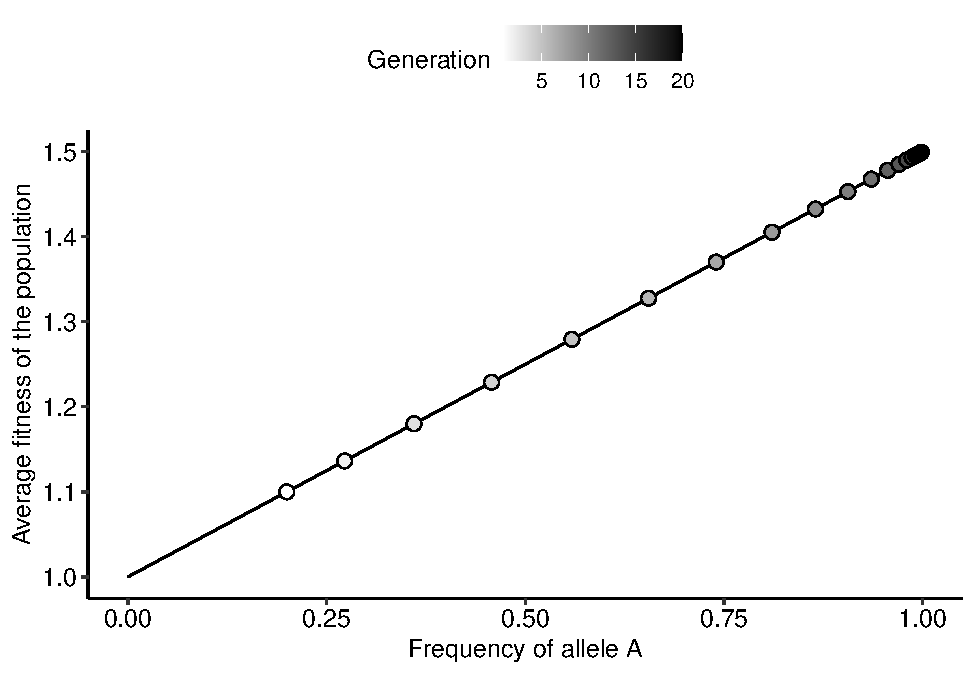
\includegraphics[width=0.65\linewidth,height=0.65\textheight]{_main_files/figure-latex/unnamed-chunk-8-1}

From the figure above we can visualize the result that we obtained from Wright's equation: when fitness is frequency independent, evolution by natural selection favors adaptations and increases the average fitness of a population. But what about when fitness is frequency-dependent? As we did before, we can adapt our code to incorporate different assumptions about fitness. For instance, we could build the fitness landscape for the same scenario that we already simulated, where fitness can decrease depending on the frequency of the alleles with a strength of \(\alpha\) and \(\beta\). The code below simulates this scenario and build the fitness landscape of the population.

\begin{Shaded}
\begin{Highlighting}[]
\NormalTok{evo\_landscape}\OtherTok{\textless{}{-}}\ControlFlowTok{function}\NormalTok{(tmax, p0, alpha, beta)\{ }\CommentTok{\#Defining the function and the input arguments}
  
\NormalTok{p\_theo }\OtherTok{=} \FunctionTok{seq}\NormalTok{(}\DecValTok{0}\NormalTok{, }\DecValTok{1}\NormalTok{, }\FloatTok{0.001}\NormalTok{) }\CommentTok{\# Defining the theoretical values of p to build the fitness landscape}
\NormalTok{wA\_theo }\OtherTok{=} \DecValTok{1} \SpecialCharTok{{-}}\NormalTok{ (alpha}\SpecialCharTok{*}\NormalTok{p\_theo) }\CommentTok{\# Defining the fitness function of A}
\NormalTok{wB\_theo }\OtherTok{=} \DecValTok{1} \SpecialCharTok{{-}}\NormalTok{ (beta}\SpecialCharTok{*}\NormalTok{(}\DecValTok{1}\SpecialCharTok{{-}}\NormalTok{p\_theo)) }\CommentTok{\# Defining the fitness function of A}
\NormalTok{w\_avg\_theo }\OtherTok{=}\NormalTok{ p\_theo}\SpecialCharTok{*}\NormalTok{wA\_theo }\SpecialCharTok{+}\NormalTok{ (}\DecValTok{1}\SpecialCharTok{{-}}\NormalTok{p\_theo)}\SpecialCharTok{*}\NormalTok{wB\_theo }\CommentTok{\#Computing the average fitness}
\NormalTok{land }\OtherTok{=} \FunctionTok{data.frame}\NormalTok{(p\_theo, w\_avg\_theo) }\CommentTok{\#Building a data frame with values of p and the corresponding average fitness}
  
\NormalTok{dp }\OtherTok{=} \FunctionTok{c}\NormalTok{() }\CommentTok{\#Creating the vector to store the outcome}
\NormalTok{dw }\OtherTok{=} \FunctionTok{c}\NormalTok{() }\CommentTok{\#Creating a vector to keep track of the average fitness along the evolutionary dynamics}
\NormalTok{dp[}\DecValTok{1}\NormalTok{]}\OtherTok{\textless{}{-}}\NormalTok{p0 }\CommentTok{\#Setting the initial frequency of p}
  
  \ControlFlowTok{for}\NormalTok{(t }\ControlFlowTok{in} \DecValTok{1}\SpecialCharTok{:}\NormalTok{(tmax}\DecValTok{{-}1}\NormalTok{))\{ }\CommentTok{\#Setting up the for loop}
  
\NormalTok{  p }\OtherTok{=}\NormalTok{ dp[t] }\CommentTok{\# Setting current frequencies}
\NormalTok{  wA }\OtherTok{=} \DecValTok{1}\SpecialCharTok{{-}}\NormalTok{(alpha}\SpecialCharTok{*}\NormalTok{p) }\CommentTok{\#Computing the fitness of A at the current generation}
\NormalTok{  wB }\OtherTok{=} \DecValTok{1}\SpecialCharTok{{-}}\NormalTok{(beta}\SpecialCharTok{*}\NormalTok{(}\DecValTok{1}\SpecialCharTok{{-}}\NormalTok{p)) }\CommentTok{\#Computing the fitness of B at the current generation}
\NormalTok{  w\_avg }\OtherTok{=}\NormalTok{ p}\SpecialCharTok{*}\NormalTok{wA }\SpecialCharTok{+}\NormalTok{ (}\DecValTok{1}\SpecialCharTok{{-}}\NormalTok{p)}\SpecialCharTok{*}\NormalTok{wB }\CommentTok{\# Computing average fitness}
\NormalTok{  dw[t] }\OtherTok{=}\NormalTok{ w\_avg}
\NormalTok{  dp[t}\SpecialCharTok{+}\DecValTok{1}\NormalTok{]}\OtherTok{=}\NormalTok{ p }\SpecialCharTok{+}\NormalTok{ (p}\SpecialCharTok{*}\NormalTok{(}\DecValTok{1}\SpecialCharTok{{-}}\NormalTok{p)}\SpecialCharTok{*}\NormalTok{(wA}\SpecialCharTok{{-}}\NormalTok{wB)}\SpecialCharTok{/}\NormalTok{w\_avg) }\CommentTok{\#Updating frequency values}
  
\NormalTok{\}}
\NormalTok{  dw[tmax] }\OtherTok{=}\NormalTok{  dp[tmax]}\SpecialCharTok{*}\NormalTok{wA }\SpecialCharTok{+}\NormalTok{ (}\DecValTok{1}\SpecialCharTok{{-}}\NormalTok{dp[tmax])}\SpecialCharTok{*}\NormalTok{wB }\CommentTok{\#Computing average fitness for the final time step}
\NormalTok{  r }\OtherTok{=} \FunctionTok{data.frame}\NormalTok{(}\AttributeTok{dp=}\NormalTok{dp, dw, }\AttributeTok{t=}\DecValTok{1}\SpecialCharTok{:}\NormalTok{tmax) }\CommentTok{\# Building the data frame}
  
  \FunctionTok{return}\NormalTok{(}\FunctionTok{list}\NormalTok{(land, r)) }\CommentTok{\# Returning a list with the data frame of the dynamics and the landscape, respectively}
  
\NormalTok{\}}

\CommentTok{\# Running the function:}

\NormalTok{r\_list }\OtherTok{=} \FunctionTok{evo\_landscape}\NormalTok{(}\AttributeTok{tmax=}\DecValTok{50}\NormalTok{, }\AttributeTok{p0=}\FloatTok{0.2}\NormalTok{, }\AttributeTok{alpha=}\FloatTok{0.1}\NormalTok{, }\AttributeTok{beta=}\FloatTok{0.2}\NormalTok{)}

\CommentTok{\# Plotting the landscape and how the population moves over generations}

\FunctionTok{ggplot}\NormalTok{()}\SpecialCharTok{+}
  \FunctionTok{geom\_line}\NormalTok{(}\AttributeTok{data=}\NormalTok{r\_list[[}\DecValTok{1}\NormalTok{]], }\FunctionTok{aes}\NormalTok{(}\AttributeTok{x=}\NormalTok{p\_theo, }\AttributeTok{y=}\NormalTok{w\_avg\_theo))}\SpecialCharTok{+}
  \FunctionTok{geom\_point}\NormalTok{(}\AttributeTok{data=}\NormalTok{r\_list[[}\DecValTok{2}\NormalTok{]], }\FunctionTok{aes}\NormalTok{(}\AttributeTok{x=}\NormalTok{dp, }\AttributeTok{y=}\NormalTok{dw, }\AttributeTok{fill=}\NormalTok{t), }\AttributeTok{color=}\StringTok{"black"}\NormalTok{, }\AttributeTok{shape=}\DecValTok{21}\NormalTok{, }\AttributeTok{size=}\DecValTok{3}\NormalTok{)}\SpecialCharTok{+}
  \FunctionTok{scale\_fill\_gradientn}\NormalTok{(}\AttributeTok{colors=}\FunctionTok{c}\NormalTok{(}\StringTok{"white"}\NormalTok{, }\StringTok{"black"}\NormalTok{))}\SpecialCharTok{+}
  \FunctionTok{labs}\NormalTok{(}\AttributeTok{fill=}\StringTok{"Generation"}\NormalTok{)}\SpecialCharTok{+}
  \FunctionTok{xlab}\NormalTok{(}\StringTok{"Frequency of allele A"}\NormalTok{)}\SpecialCharTok{+}\FunctionTok{ylab}\NormalTok{(}\StringTok{"Average fitness of the population"}\NormalTok{)}\SpecialCharTok{+}
  \FunctionTok{theme\_pubr}\NormalTok{()}
\end{Highlighting}
\end{Shaded}

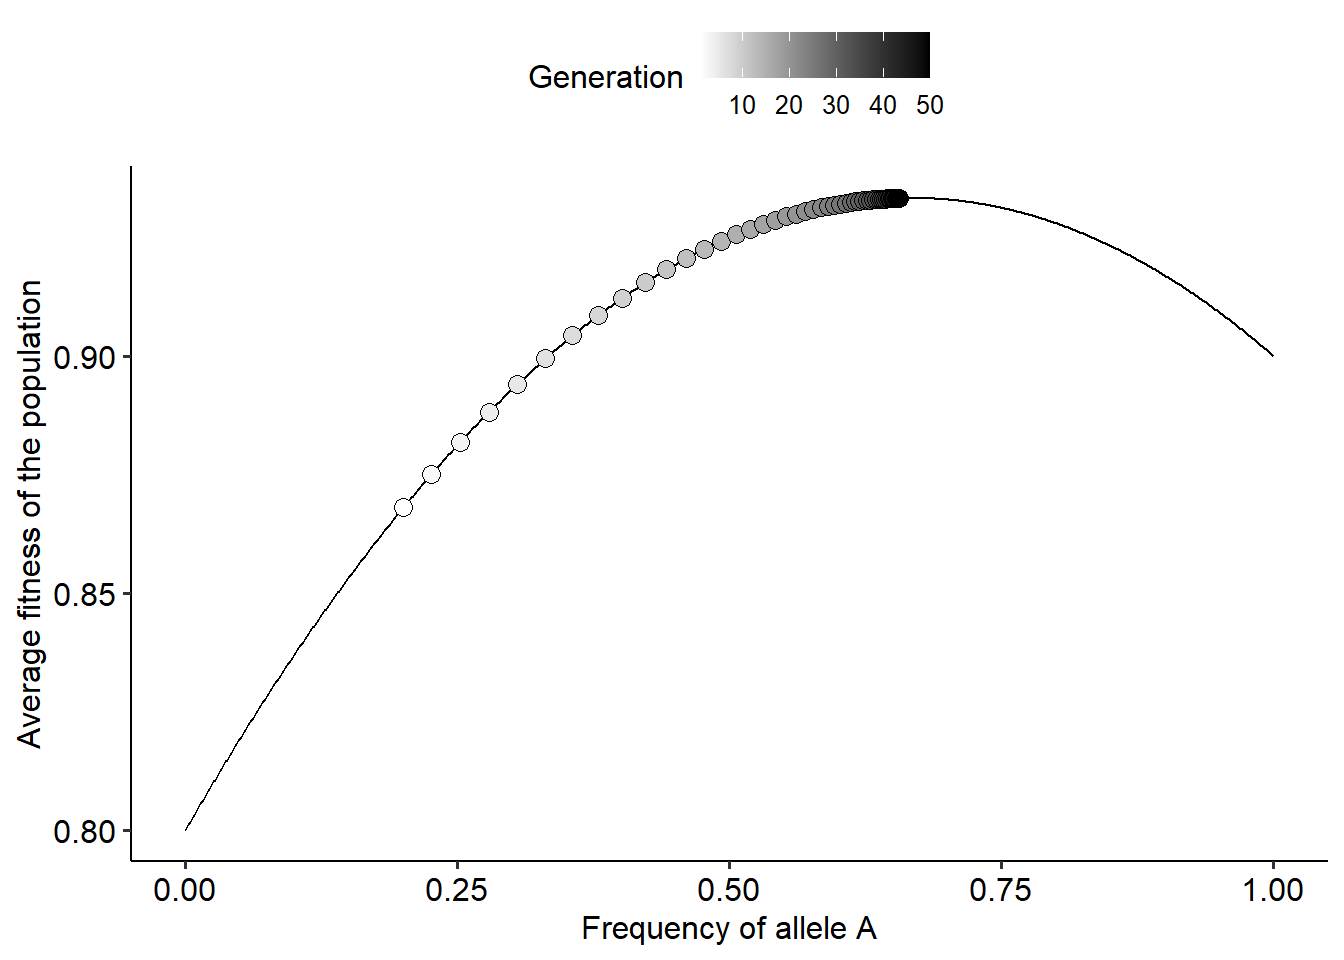
\includegraphics[width=0.65\linewidth,height=0.65\textheight]{_main_files/figure-latex/unnamed-chunk-9-1}

Using this new function, explore how different values of \(\alpha\) and \(\beta\) change the shape of the landscape. Try to answer the following questions:

\begin{enumerate}
\def\labelenumi{\arabic{enumi}.}
\tightlist
\item
  How the fitness landscape changes when fitness is a frequency-independent versus frequency-dependent?
\item
  How the values of \(\alpha\) and \(\beta\) modify the shape of the fitness landscape?
\item
  Challenge: similar to how we did it for frequency-independent fitness values, try to interpret the shape of the landscape in terms of the equation of \(\overline{W}\) as a function of \(p\).
\end{enumerate}

\hypertarget{exercise-simulating-evolution-using-the-price-theorem}{%
\chapter{Exercise: Simulating evolution using the Price theorem}\label{exercise-simulating-evolution-using-the-price-theorem}}

\hypertarget{simulating-evolutionary-changes-in-allele-frequencies-1}{%
\section{Simulating evolutionary changes in allele frequencies}\label{simulating-evolutionary-changes-in-allele-frequencies-1}}

In our second lecture we studied and derived the Price theorem (Price 1970) that can be used to predict how the mean value of any measurable property of a population change from one generation to the other. For this exercise section, we will use the Price theorem to gain more intuition about how the moments of the distribution of traits in a population can evolve by natural selection. Building upon the core results of the theorem, We will also study how we can predict the mode of selection in a population (directional, stabilizing and disruptive) using linear regressions.

We begin with the Price theorem, that can be expressed as the following equation (Rice 2005):

\[
\Delta \overline{z}=\frac{1}{\overline{W}}\left[Cov(W, z) + E(W\overline{\delta}) \right]
\] As we studied during the lecture, the equation is comprised of two terms. The first term, \(\frac{1}{\overline{W}}Cov(W, z)\) encompass the changes due to differential survival and reproduction, while the second one, comprises changes resulting from any process involved in reproduction. For this exercise section we will assume that \(E(W\overline{\delta})=0\) and will work with the simplified version of the Price theorem, \(\Delta \overline{z}=\frac{1}{\overline{W}}Cov(W, z)\).

We begin simulating a measurable trait, \(z\), that follows a normal distribution with mean \(\mu=5.0\) and \(\sigma^2=1.0\) in a population of 10000 individuals:

\begin{Shaded}
\begin{Highlighting}[]
\FunctionTok{library}\NormalTok{(ggplot2)}
\FunctionTok{library}\NormalTok{(ggpubr)}

\NormalTok{n}\OtherTok{=}\DecValTok{10000} \CommentTok{\#Population size}
\NormalTok{z\_u}\OtherTok{=}\DecValTok{5} \CommentTok{\#Mean trait value}
\NormalTok{z\_var}\OtherTok{=}\DecValTok{1} \CommentTok{\#Variance}
\NormalTok{z }\OtherTok{=} \FunctionTok{rnorm}\NormalTok{(n, }\AttributeTok{mean=}\NormalTok{z\_u, }\AttributeTok{sd=}\FunctionTok{sqrt}\NormalTok{(z\_var)) }\CommentTok{\#Sampling from a normal distribution with mean=5 and variance=1 (the standard deviation is equal to the square root of the variance).}

\CommentTok{\# Plotting the distribution}
\FunctionTok{ggplot}\NormalTok{(}\AttributeTok{data=}\FunctionTok{data.frame}\NormalTok{(z))}\SpecialCharTok{+}
  \FunctionTok{geom\_density}\NormalTok{(}\FunctionTok{aes}\NormalTok{(}\AttributeTok{x=}\NormalTok{z))}\SpecialCharTok{+}
  \FunctionTok{xlab}\NormalTok{(}\StringTok{"Trait value"}\NormalTok{)}\SpecialCharTok{+}\FunctionTok{ylab}\NormalTok{(}\StringTok{"Density"}\NormalTok{)}\SpecialCharTok{+}
  \FunctionTok{theme\_pubr}\NormalTok{()}
\end{Highlighting}
\end{Shaded}

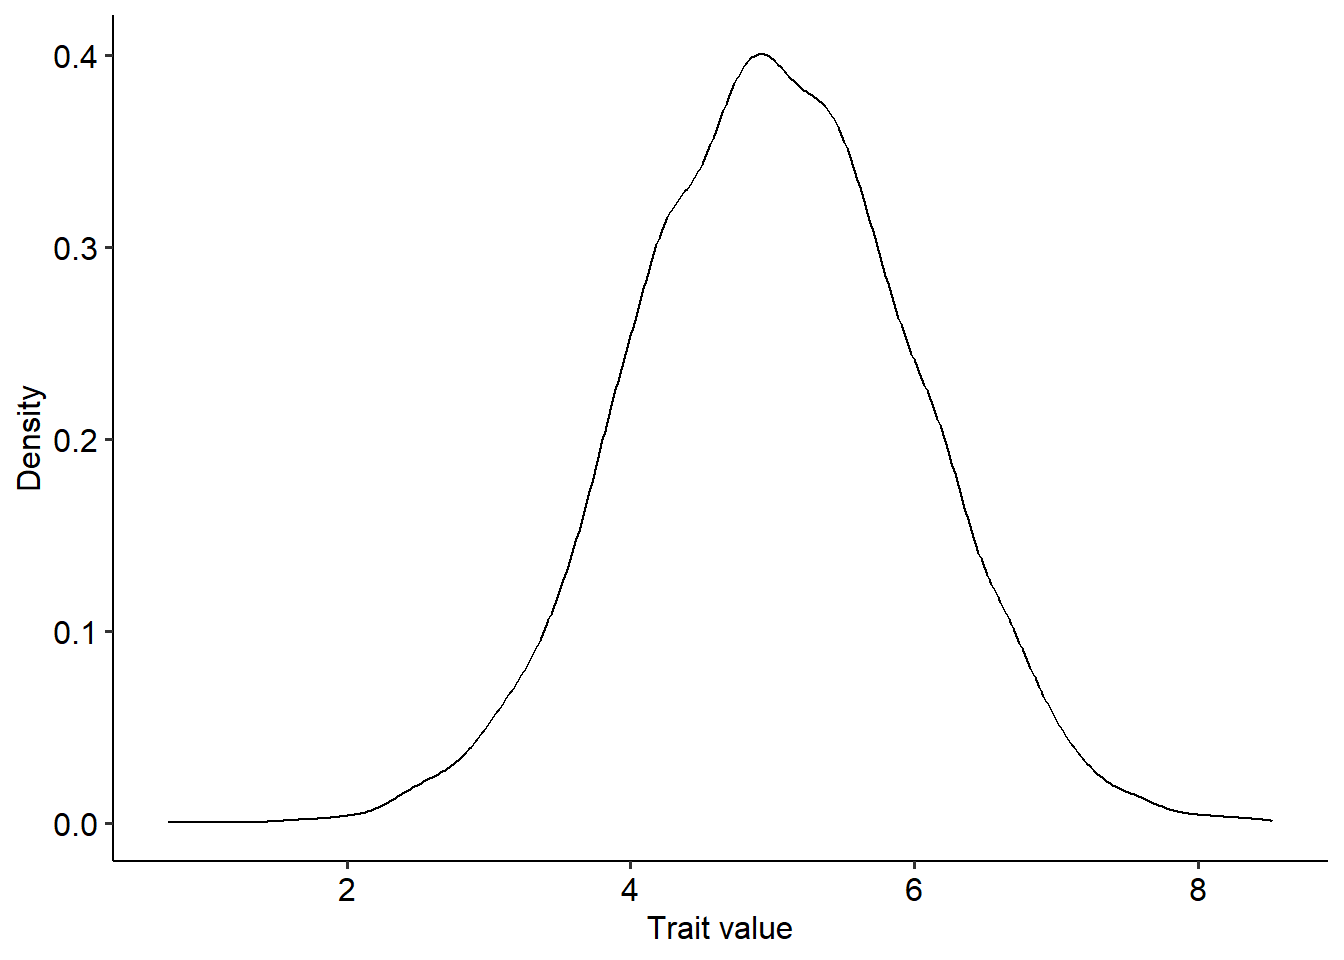
\includegraphics[width=0.65\linewidth,height=0.65\textheight]{_main_files/figure-latex/unnamed-chunk-10-1}

Now that we have a distribution of traits, we can begin to use the Price theorem to predict how the moments of this distribution can change because of differential survival and reproduction. Here we will focus on the first and second moments of the distribution - the mean and the variance - but the theorem can also be used for other higher order moments. As examples, we will use three different types of functions for how the fitness of individuals vary with trait values: (1) \(W=1+c+\epsilon\); (2) \(W=1+\beta z +\epsilon\) (3) \(W=e^{-\alpha\left(\theta-z+\epsilon\right)^2}\); where \(c\) is a constant; \(\beta\), \(\alpha\) and \(\theta\) are parameters that control the shape of the functions; and \(\epsilon\) is a small amount of random noise that we will sample from a normal distribution. In the code block below we define these functions.

\begin{Shaded}
\begin{Highlighting}[]
\CommentTok{\#Defining the parameters of the fitness functions:}

\NormalTok{e}\OtherTok{=}\FunctionTok{rnorm}\NormalTok{(n, }\AttributeTok{mean=}\DecValTok{0}\NormalTok{, }\AttributeTok{sd=}\FloatTok{0.05}\NormalTok{) }\CommentTok{\#Sampling random noise}
\NormalTok{c}\OtherTok{=}\DecValTok{1} \CommentTok{\# Parameter of fitness function (1)}
\NormalTok{beta}\OtherTok{=}\FloatTok{0.5} \CommentTok{\# Parameter of fitness functions (2)}
\NormalTok{alpha}\OtherTok{=}\FloatTok{0.5}\NormalTok{; theta}\OtherTok{=}\FloatTok{4.0} \CommentTok{\# Parameters of fitness function (3)}

\NormalTok{w1}\OtherTok{=}\DecValTok{1}\SpecialCharTok{+}\NormalTok{c}\SpecialCharTok{+}\NormalTok{e }\CommentTok{\#Fitness function (1)}
\NormalTok{w2}\OtherTok{=}\DecValTok{1}\SpecialCharTok{+}\NormalTok{beta}\SpecialCharTok{*}\NormalTok{z}\SpecialCharTok{+}\NormalTok{e }\CommentTok{\#Fitness function (2)}
\NormalTok{w3}\OtherTok{=}\DecValTok{1}\SpecialCharTok{+}\FunctionTok{exp}\NormalTok{(}\SpecialCharTok{{-}}\NormalTok{alpha}\SpecialCharTok{*}\NormalTok{(theta}\SpecialCharTok{{-}}\NormalTok{z}\SpecialCharTok{+}\NormalTok{e)}\SpecialCharTok{\^{}}\DecValTok{2}\NormalTok{) }\CommentTok{\#Fitness function (3)}
\end{Highlighting}
\end{Shaded}

Now that we have trait values and their corresponding fitness, we can use Price's theorem to predict the change in the mean and variance of the trait distribution from one generation to the other. For the mean, we need to compute the covariance between trait values and fitness, \(Cov(W,z)\), while for the variance, we need to compute the covariance between fitness and the squared deviation of trait values to the mean, \(Cov\left[W, (z-\overline{z})^2\right]\). Then, we divide the two covariances by the average fitness of the population, \(\overline{W}\). Finally, we can plot the new distribution on top of the old one. The code to perform these steps for the fitness function \(W=1+c+\epsilon\) is as follows:

\begin{Shaded}
\begin{Highlighting}[]
\NormalTok{delta\_z}\OtherTok{=}\FunctionTok{cov}\NormalTok{(w1,z)}\SpecialCharTok{/}\FunctionTok{mean}\NormalTok{(w1) }\CommentTok{\#Change in the mean of z}
\NormalTok{delta\_zvar}\OtherTok{=}\FunctionTok{cov}\NormalTok{(w1,(z}\SpecialCharTok{{-}}\FunctionTok{mean}\NormalTok{(z))}\SpecialCharTok{\^{}}\DecValTok{2}\NormalTok{)}\SpecialCharTok{/}\FunctionTok{mean}\NormalTok{(w1) }\CommentTok{\#Change in the variance of z}

\CommentTok{\# Getting new distribution of trait values}

\NormalTok{z\_new}\OtherTok{=}\FunctionTok{rnorm}\NormalTok{(n, }\AttributeTok{mean=}\NormalTok{z\_u}\SpecialCharTok{+}\NormalTok{delta\_z, }\AttributeTok{sd=}\FunctionTok{sqrt}\NormalTok{(z\_var}\SpecialCharTok{+}\NormalTok{delta\_z))}

\FunctionTok{ggplot}\NormalTok{(}\AttributeTok{data=}\FunctionTok{data.frame}\NormalTok{(}\AttributeTok{z=}\NormalTok{z, }\AttributeTok{z\_new=}\NormalTok{z\_new))}\SpecialCharTok{+}
  \FunctionTok{geom\_density}\NormalTok{(}\FunctionTok{aes}\NormalTok{(}\AttributeTok{x=}\NormalTok{z), }\AttributeTok{linetype=}\StringTok{"dashed"}\NormalTok{)}\SpecialCharTok{+}
  \FunctionTok{geom\_density}\NormalTok{(}\FunctionTok{aes}\NormalTok{(}\AttributeTok{x=}\NormalTok{z\_new))}\SpecialCharTok{+}
  \FunctionTok{xlab}\NormalTok{(}\StringTok{"Trait value"}\NormalTok{)}\SpecialCharTok{+}\FunctionTok{ylab}\NormalTok{(}\StringTok{"Counts"}\NormalTok{)}\SpecialCharTok{+}
  \FunctionTok{theme\_pubr}\NormalTok{()}
\end{Highlighting}
\end{Shaded}

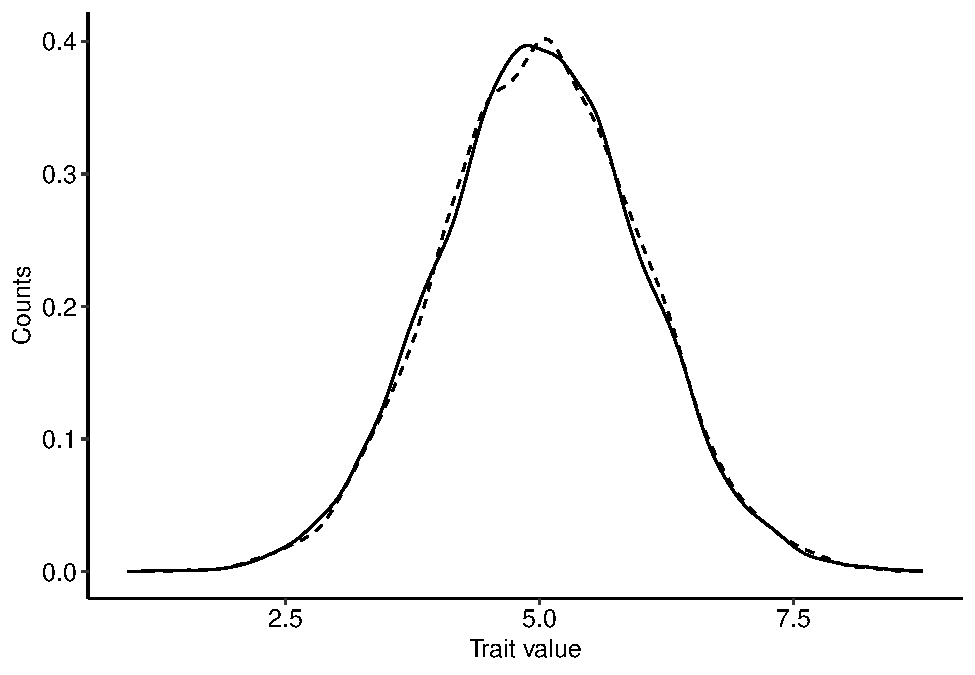
\includegraphics[width=0.65\linewidth,height=0.65\textheight]{_main_files/figure-latex/unnamed-chunk-12-1}

In the figure above, the dashed line represent the previous trait distribution, while the solid line the new one. The distributions look pretty much the same and the change in the mean and variance of the distribution of trait values is negligible. Considering the fitness function \(W=1+c+\epsilon\), try to explain why there was no change in the distribution. Use the code above to predict how the distribution changes for the other two fitness functions. What differences can you observe?

\hypertarget{the-regression-of-fitness-on-phenotypes-and-the-modes-of-selection}{%
\section{The regression of fitness on phenotypes and the modes of selection}\label{the-regression-of-fitness-on-phenotypes-and-the-modes-of-selection}}

Now that we know how to compute the change in the mean and variance of the distribution of traits in a population, we can try to gain intuition about the different modes of selection. To do so, we will use the two remaining fitness functions, \(W=1+\beta z +\epsilon\) and \(W=e^{-\alpha\left(\theta-z\right)^2+\epsilon}\). In the lecture we studied that the Price theorem can be rewritten as a regression of fitness on trait values, as follows:

\[
\Delta \overline{z}=\frac{1}{\overline{W}}\beta_{(W,z)} Var(z)
\] From the above equation, we can study how natural selection drives the evolution of the mean and the variance of trait values with the corresponding regression coefficients. These regression coefficients can be computed from the covariances and variances as \(\beta_{(W,z)}=\frac{Cov(W,z)}{Var(z)}\). When the trait itself is \((z-\overline{z})^2\), the regression coefficient can be computed as \(\beta_{\left[W,(z-\overline{z})^2\right]}=\frac{Cov\left[W,(z-\overline{z})^2\right]}{Var\left[(z-\overline{z})^2\right]}\). When the regression coefficient of fitness on the trait \(z\) is non zero, the trait is under \emph{directional selection}. Similarly, if the regression coefficient of fitness on \((z-\overline{z})^2\) is non zero, the trait is either under \emph{stabilizing selection} (\(\beta_{\left[W,(z-\overline{z})^2\right]}<0\)) or \emph{disruptive selection} (\(\beta_{\left[W,(z-\overline{z})^2\right]}>0\)). For the fitness functions that we are going to use in this part of the exercise section, we can visually assess the modes of selection acting on trait \(z\). The code to do so is reproduced below:

\begin{Shaded}
\begin{Highlighting}[]
\FunctionTok{library}\NormalTok{(patchwork)}

\CommentTok{\# Creating a data frame with variables z, the squared deviations of z to the mean, and the fitness of individuals in the population when using fitness functions (2) and (3)}

\NormalTok{z\_df }\OtherTok{=} \FunctionTok{data.frame}\NormalTok{(}\AttributeTok{z=}\NormalTok{z, }\AttributeTok{z2=}\NormalTok{(z}\SpecialCharTok{{-}}\FunctionTok{mean}\NormalTok{(z))}\SpecialCharTok{\^{}}\DecValTok{2}\NormalTok{, }\AttributeTok{w2=}\NormalTok{w2, }\AttributeTok{w3=}\NormalTok{w3)}

\CommentTok{\# Creating plots with the regression between z and w2, as well as (z{-}mean(z))\^{}2 for w2}

\NormalTok{p1 }\OtherTok{=} \FunctionTok{ggplot}\NormalTok{(}\AttributeTok{data=}\NormalTok{z\_df, }\FunctionTok{aes}\NormalTok{(}\AttributeTok{x=}\NormalTok{z, }\AttributeTok{y=}\NormalTok{w2))}\SpecialCharTok{+}
  \FunctionTok{geom\_point}\NormalTok{()}\SpecialCharTok{+}
  \FunctionTok{xlab}\NormalTok{(}\StringTok{"Trait values"}\NormalTok{)}\SpecialCharTok{+}\FunctionTok{ylab}\NormalTok{(}\StringTok{"Fitness (function \#2)"}\NormalTok{)}\SpecialCharTok{+}
  \FunctionTok{geom\_smooth}\NormalTok{(}\AttributeTok{method=}\StringTok{"lm"}\NormalTok{, }\AttributeTok{se=}\NormalTok{F)}\SpecialCharTok{+}
  \FunctionTok{theme\_pubr}\NormalTok{()}

\NormalTok{p2 }\OtherTok{=} \FunctionTok{ggplot}\NormalTok{(}\AttributeTok{data=}\NormalTok{z\_df, }\FunctionTok{aes}\NormalTok{(}\AttributeTok{x=}\NormalTok{z2, }\AttributeTok{y=}\NormalTok{w2))}\SpecialCharTok{+}
  \FunctionTok{geom\_point}\NormalTok{()}\SpecialCharTok{+}
  \FunctionTok{xlab}\NormalTok{(}\StringTok{"Squared deviation of trait values to the mean"}\NormalTok{)}\SpecialCharTok{+}\FunctionTok{ylab}\NormalTok{(}\StringTok{"Fitness (function \#2)"}\NormalTok{)}\SpecialCharTok{+}
  \FunctionTok{geom\_smooth}\NormalTok{(}\AttributeTok{method=}\StringTok{"lm"}\NormalTok{, }\AttributeTok{se=}\NormalTok{F)}\SpecialCharTok{+}
  \FunctionTok{theme\_pubr}\NormalTok{()}

\CommentTok{\# Creating plots with the regression between z and w2, as well as (z{-}mean(z))\^{}2 for w3}

\NormalTok{p3 }\OtherTok{=} \FunctionTok{ggplot}\NormalTok{(}\AttributeTok{data=}\NormalTok{z\_df, }\FunctionTok{aes}\NormalTok{(}\AttributeTok{x=}\NormalTok{z, }\AttributeTok{y=}\NormalTok{w3))}\SpecialCharTok{+}
  \FunctionTok{geom\_point}\NormalTok{()}\SpecialCharTok{+}
  \FunctionTok{xlab}\NormalTok{(}\StringTok{"Trait values"}\NormalTok{)}\SpecialCharTok{+}\FunctionTok{ylab}\NormalTok{(}\StringTok{"Fitness (function \#3)"}\NormalTok{)}\SpecialCharTok{+}
  \FunctionTok{geom\_smooth}\NormalTok{(}\AttributeTok{method=}\StringTok{"lm"}\NormalTok{, }\AttributeTok{se=}\NormalTok{F)}\SpecialCharTok{+}
  \FunctionTok{theme\_pubr}\NormalTok{()}

\NormalTok{p4 }\OtherTok{=} \FunctionTok{ggplot}\NormalTok{(}\AttributeTok{data=}\NormalTok{z\_df, }\FunctionTok{aes}\NormalTok{(}\AttributeTok{x=}\NormalTok{z2, }\AttributeTok{y=}\NormalTok{w3))}\SpecialCharTok{+}
  \FunctionTok{geom\_point}\NormalTok{()}\SpecialCharTok{+}
  \FunctionTok{xlab}\NormalTok{(}\StringTok{"Squared deviation of trait values to the mean"}\NormalTok{)}\SpecialCharTok{+}\FunctionTok{ylab}\NormalTok{(}\StringTok{"Fitness (function \#3)"}\NormalTok{)}\SpecialCharTok{+}
  \FunctionTok{geom\_smooth}\NormalTok{(}\AttributeTok{method=}\StringTok{"lm"}\NormalTok{, }\AttributeTok{se=}\NormalTok{F)}\SpecialCharTok{+}
  \FunctionTok{theme\_pubr}\NormalTok{()}

\CommentTok{\# Combining all plots using the patchwork package}

\NormalTok{p1}\SpecialCharTok{+}\NormalTok{p2}\SpecialCharTok{+}\NormalTok{p3}\SpecialCharTok{+}\NormalTok{p4 }\SpecialCharTok{+} \FunctionTok{plot\_annotation}\NormalTok{(}\AttributeTok{tag\_levels=}\FunctionTok{c}\NormalTok{(}\StringTok{"a"}\NormalTok{))}
\end{Highlighting}
\end{Shaded}

\begin{verbatim}
## `geom_smooth()` using formula = 'y ~ x'
## `geom_smooth()` using formula = 'y ~ x'
## `geom_smooth()` using formula = 'y ~ x'
## `geom_smooth()` using formula = 'y ~ x'
\end{verbatim}

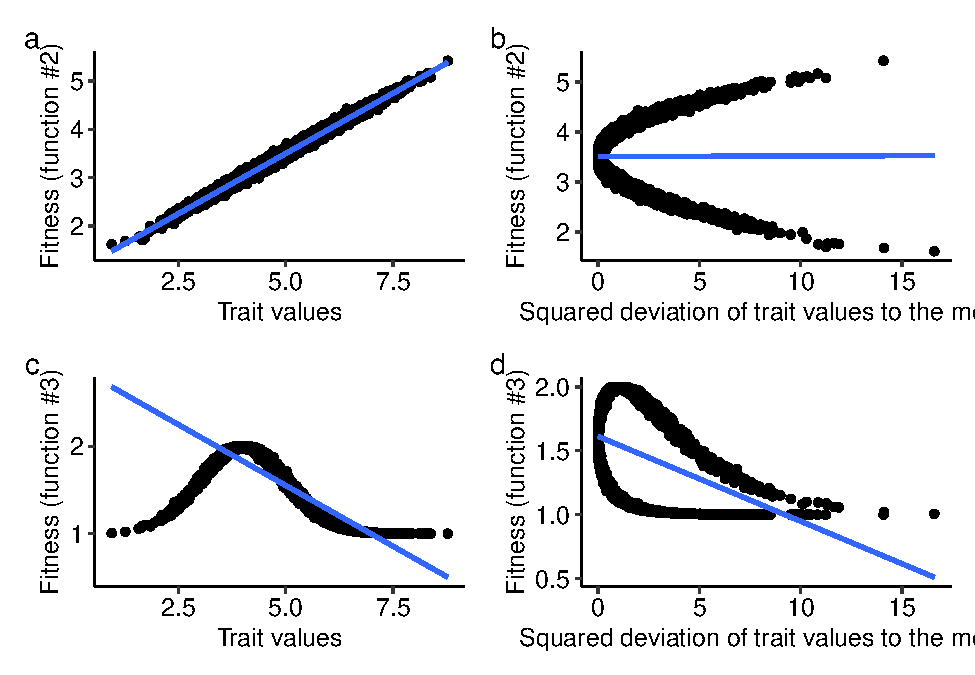
\includegraphics[width=0.65\linewidth,height=0.65\textheight]{_main_files/figure-latex/unnamed-chunk-13-1}

From the plots above, try to answer the following questions:

\begin{enumerate}
\def\labelenumi{\arabic{enumi}.}
\tightlist
\item
  What are the modes of selection for the fitness functions (2) and (3)?
\item
  What would be a possible biological interpretation of the parameter \(\theta\) in the fitness function \(W=e^{-\alpha\left(\theta-z+\epsilon\right)^2}\)?
\item
  Try changing both \(\theta\) (e.g.~to \(\theta=6.0\) instead of \(\theta=4.0\)) and \(\alpha\). How these parameters change the relationship between fitness, trait values, and the regression coefficients?
\end{enumerate}

\hypertarget{exercise-simulating-evolution-using-landes-equation}{%
\chapter{Exercise: Simulating evolution using Lande's equation}\label{exercise-simulating-evolution-using-landes-equation}}

\hypertarget{simulating-evolutionary-changes-in-continuous-traits}{%
\section{Simulating evolutionary changes in continuous traits}\label{simulating-evolutionary-changes-in-continuous-traits}}

Our third lecture introduced the classical equation in quantitative genetics derived by \href{https://onlinelibrary.wiley.com/doi/10.1111/j.1558-5646.1976.tb00911.x}{Russel Lande (1976)}. After studying and going through the steps to derive this equation, here we will use it to simulate evolutionary changes in continuously varying traits. Lande's equation relates how the mean value of a continuous trait in a population (\(\overline{z}\)) changes from one generation to the other in response to the available variance of the trait in the population (\(\sigma^{2}_{z}\)), its heritability, \(h^2\), and direction and intensity of natural selection. The direction and intensity of selection on the trait is mathematically described by the selection gradient, \(\frac{\partial ln\overline{W}}{\partial \overline{z}}\). These two components underly Lande's equation and can be used to predict evolutionary changes in \(\overline{z}\) as follows:

\[
\Delta \overline{z}=h^2 \sigma^{2}_{z}\frac{\partial ln\overline{W}}{\partial \overline{z}}
\]

There are two main approaches that we can use to model evolutionary changes using Lande's equation. For the first one, our starting point is a function describing how the fitness of individuals vary with trait values. We next use this function to derive a new one, describing how the mean fitness of the population depends on the mean values of traits. Finally, we derive the selection gradient which can then, be plugged in into Lande's equation. The second approach is directly assuming a function for the selection gradient. Here, we will use the first approach, but we will also see how to use the second one in block 2 of the course.

Thus, our first step is to define a function, \(W(z)\), describing how fitness of individuals vary with trait values. We will use the two fitness functions that are similar to the ones used in the previous exercise section, as follows:

\[\begin{align}
W_{1}(z) &= 1+\beta z \\
W_{2}(z) &= e^{-\alpha\left(\theta-z\right)^2}
\end{align}\]

We now need to derive how mean fitness changes relative to mean trait values. To do so, we need to compute the expected value of the fitness function of individuals. For linear functions of random variable, such as \(W_{1}(z)\), computing an expected value is straightforward because of two identities: \(E[aX]=aE[X]\) and \(E[X+b]=E[X]+b\). For our function \(W_{1}(z)\), we can apply these two identities as follows:

\[
E[1+\beta z] = 1+E[\beta z]=1+\beta E[z]=1+\beta \overline{z}
\] where we used the equivalence \(E[z]=\overline{z}\) just to simplify the notation. For the second fitness function, \(W_{2}(z)\), we need to rely on an approximation to compute the expected value. When \(z\) is normally distributed (as it needs to be when applying Lande's equation), with small values of \(\alpha\) or variance, \(\sigma^2\), we can approximate this expectation as follows:

\[
E[e^{-\alpha\left(\theta-z\right)^2}] \approx e^{-\alpha\left[\left(\theta-\overline{z}\right)^2 + \sigma^2\right]}
\]

We will not cover the approximation in the course, but it comes from how we can approximate \(E[ln f(X)]\) as \(lnE[f(X)]\) under the assumptions mentioned above (\href{https://pubmed.ncbi.nlm.nih.gov/3744046/}{Barton 1986}).

Our last step is to derive the selection gradient. For that we need to apply the natural logarithm to the functions above and compute their derivatives relative to the mean trait value. Computing derivatives is very straightforward when you are familiar with all of the rules. If you are not familiar with computing derivatives, we can do it using the function D() in R. To use this R function, we just need to define an expression and the variable that we wish to compute the derivative in that expression. The code to do so for the fitness function \(\overline{W}_{1}(\overline{z})\) is as follows:

\begin{Shaded}
\begin{Highlighting}[]
\NormalTok{dw1}\OtherTok{=}\FunctionTok{D}\NormalTok{(}\FunctionTok{expression}\NormalTok{(}\FunctionTok{log}\NormalTok{(}\DecValTok{1}\SpecialCharTok{+}\NormalTok{beta}\SpecialCharTok{*}\NormalTok{z)), }\StringTok{"z"}\NormalTok{)}
\FunctionTok{print}\NormalTok{(dw1)}
\end{Highlighting}
\end{Shaded}

\begin{verbatim}
## beta/(1 + beta * z)
\end{verbatim}

As you can see, the derivative is equal to \(\frac{\beta}{1+\beta \overline{z}}\). We can repeat the same process for second fitness function, \(e^{-\alpha\left[\left(\theta-\overline{z}\right)^2 + \sigma^2\right]}\). Since we are computing the derivative of the natural logarithm of this function, we can simplify it as \(lnW_{2}(\overline{z})=-\alpha\left[\left(\theta-\overline{z}\right)^2 + \sigma^2\right]\) and use the simplified function to compute the derivative, as follows:

\begin{Shaded}
\begin{Highlighting}[]
\NormalTok{dw2}\OtherTok{=}\FunctionTok{D}\NormalTok{(}\FunctionTok{expression}\NormalTok{(}\SpecialCharTok{{-}}\NormalTok{a}\SpecialCharTok{*}\NormalTok{((theta}\SpecialCharTok{{-}}\NormalTok{z)}\SpecialCharTok{\^{}}\DecValTok{2}\SpecialCharTok{+}\NormalTok{v)), }\StringTok{"z"}\NormalTok{) }\CommentTok{\#v here corresponds to the variance in the equation}
\FunctionTok{print}\NormalTok{(dw2)}
\end{Highlighting}
\end{Shaded}

\begin{verbatim}
## a * (2 * (theta - z))
\end{verbatim}

which evaluates to \(2\alpha (\theta-\overline{z})\). Now we have everything that we need to model how the mean value of the trait, \(\overline{z}\), changes over generations in the population. We will begin with how \(\overline{z}\) changes when we use the first fitness function. Plugging the selection gradient that we computed above for this fitness function in Lande's equation, the equation that we need to iterate over is the following one:

\[
\overline{z}^{(t+1)}=\overline{z}^{(t)}+ h^2 \sigma^{2}_{z}\frac{\beta}{1+\beta \overline{z}^{(t)}}
\]

Thus, as we did in the first exercise section, we need to define:

\begin{enumerate}
\def\labelenumi{\arabic{enumi}.}
\tightlist
\item
  A vector that will store trait values over time.
\item
  The initial trait value in the population.
\item
  The parameters of the model, such as the number of generations that we will simulate, \(t_{max}\), \(\beta\), \(\sigma^{2}_{z}\) and \(h^2\).
\end{enumerate}

Then, after defining all of the parameters we iterate over the equation using a for loop. The code to perform these steps are as follows:

\begin{Shaded}
\begin{Highlighting}[]
\NormalTok{dz }\OtherTok{=} \FunctionTok{c}\NormalTok{() }\CommentTok{\#Defining vector to store trait values over time}
\NormalTok{z0 }\OtherTok{=} \DecValTok{1} \CommentTok{\#Defining initial trait value in the population}
\NormalTok{dz[}\DecValTok{1}\NormalTok{] }\OtherTok{=}\NormalTok{ z0 }\CommentTok{\#Defining initial trait value in the population}

\NormalTok{tmax}\OtherTok{=}\DecValTok{100} \CommentTok{\# Number of generations}
\NormalTok{varz}\OtherTok{=}\FloatTok{0.1} \CommentTok{\# Phenotypic variance}
\NormalTok{h }\OtherTok{=} \FloatTok{0.1} \CommentTok{\# Heritability}
\NormalTok{beta}\OtherTok{=}\FloatTok{0.5} \CommentTok{\#Parameter beta}

\ControlFlowTok{for}\NormalTok{(t }\ControlFlowTok{in} \DecValTok{1}\SpecialCharTok{:}\NormalTok{(tmax}\DecValTok{{-}1}\NormalTok{))\{ }\CommentTok{\#Setting up the for loop}
  
\NormalTok{  z }\OtherTok{=}\NormalTok{ dz[t] }\CommentTok{\# Setting current trait values}
\NormalTok{  dlnw }\OtherTok{=}\NormalTok{ (beta}\SpecialCharTok{/}\NormalTok{(}\DecValTok{1}\SpecialCharTok{+}\NormalTok{beta}\SpecialCharTok{*}\NormalTok{z))  }\CommentTok{\#Computing the selection gradient of fitness function 1}
\NormalTok{  dz[t}\SpecialCharTok{+}\DecValTok{1}\NormalTok{]}\OtherTok{=}\NormalTok{ z }\SpecialCharTok{+}\NormalTok{ h}\SpecialCharTok{*}\NormalTok{varz}\SpecialCharTok{*}\NormalTok{dlnw }\CommentTok{\#Updating trait values using Lande\textquotesingle{}s equation}
  
\NormalTok{\}}
\end{Highlighting}
\end{Shaded}

Now, as we did before, we can put the above code inside a function to make it easier to explore the simulations and plot the results.

\begin{Shaded}
\begin{Highlighting}[]
\FunctionTok{library}\NormalTok{(ggplot2)}
\FunctionTok{library}\NormalTok{(ggpubr)}

\NormalTok{evo\_simulation}\OtherTok{\textless{}{-}}\ControlFlowTok{function}\NormalTok{(tmax, z0, varz, h, beta)\{}

\NormalTok{dz }\OtherTok{=} \FunctionTok{c}\NormalTok{() }\CommentTok{\#Defining vector to store trait values over time}
\NormalTok{dz[}\DecValTok{1}\NormalTok{] }\OtherTok{=}\NormalTok{ z0 }\CommentTok{\#Defining initial trait value in the population}

\ControlFlowTok{for}\NormalTok{(t }\ControlFlowTok{in} \DecValTok{1}\SpecialCharTok{:}\NormalTok{(tmax}\DecValTok{{-}1}\NormalTok{))\{ }\CommentTok{\#Setting up the for loop}
  
\NormalTok{  z }\OtherTok{=}\NormalTok{ dz[t] }\CommentTok{\# Setting current trait values}
\NormalTok{  dlnw }\OtherTok{=}\NormalTok{ (beta}\SpecialCharTok{/}\NormalTok{(}\DecValTok{1}\SpecialCharTok{+}\NormalTok{beta}\SpecialCharTok{*}\NormalTok{z))  }\CommentTok{\#Computing the selection gradient of fitness function 1}
\NormalTok{  dz[t}\SpecialCharTok{+}\DecValTok{1}\NormalTok{]}\OtherTok{=}\NormalTok{ z }\SpecialCharTok{+}\NormalTok{ h}\SpecialCharTok{*}\NormalTok{varz}\SpecialCharTok{*}\NormalTok{dlnw }\CommentTok{\#Updating trait values using Lande\textquotesingle{}s equation}
  
\NormalTok{\}}

\NormalTok{r }\OtherTok{=} \FunctionTok{data.frame}\NormalTok{(}\AttributeTok{dz=}\NormalTok{dz, }\AttributeTok{t=}\DecValTok{1}\SpecialCharTok{:}\NormalTok{tmax) }\CommentTok{\# Building the data frame with trait values over time}
  
\FunctionTok{return}\NormalTok{(r)}

\NormalTok{\}}

\CommentTok{\# Running the function to test it:}

\NormalTok{r }\OtherTok{=} \FunctionTok{evo\_simulation}\NormalTok{(}\AttributeTok{tmax=}\DecValTok{100}\NormalTok{, }\AttributeTok{z0=}\DecValTok{1}\NormalTok{, }\AttributeTok{h=}\FloatTok{0.1}\NormalTok{, }\AttributeTok{varz=}\FloatTok{0.1}\NormalTok{, }\AttributeTok{beta=}\FloatTok{0.5}\NormalTok{)}

\CommentTok{\# Plotting the result}

\FunctionTok{ggplot}\NormalTok{()}\SpecialCharTok{+}
  \FunctionTok{geom\_line}\NormalTok{(}\AttributeTok{data=}\NormalTok{r, }\FunctionTok{aes}\NormalTok{(}\AttributeTok{x=}\NormalTok{t, }\AttributeTok{y=}\NormalTok{dz))}\SpecialCharTok{+}
  \FunctionTok{xlab}\NormalTok{(}\StringTok{"Generation"}\NormalTok{)}\SpecialCharTok{+}\FunctionTok{ylab}\NormalTok{(}\StringTok{"Average trait value in the population"}\NormalTok{)}\SpecialCharTok{+}
  \FunctionTok{theme\_pubr}\NormalTok{()}
\end{Highlighting}
\end{Shaded}

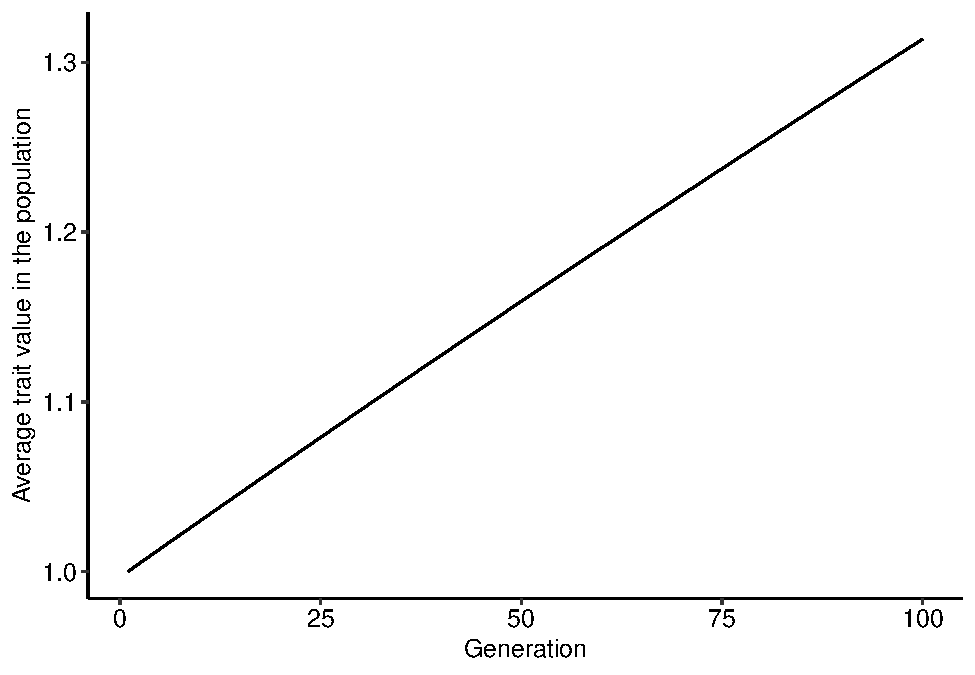
\includegraphics[width=0.65\linewidth,height=0.65\textheight]{_main_files/figure-latex/unnamed-chunk-17-1}

Using the function above, explore how different parameter values change the outcome of the evolutionary dynamics. Try to think about why we have this outcome in face of the fitness function that we are using.

\hypertarget{simulating-the-adaptive-landscape-of-a-continuous-trait}{%
\section{Simulating the adaptive landscape of a continuous trait}\label{simulating-the-adaptive-landscape-of-a-continuous-trait}}

Before proceeding to the second fitness function, we can gain more intuition about the outcome of the evolutionary dynamics when we visualize the fitness landscape of the trait. To do so, we will repeat a similar procedure to what we have already done in the first exercise section. We will go through the following steps:

\begin{enumerate}
\def\labelenumi{\arabic{enumi}.}
\item
  Build a vector containing many different values of \(\overline{z}\).
\item
  Compute the average fitness of the population, \(\overline{W}\), for each of these values of \(\overline{z}\) using the fitness function.
\item
  Plot and visualize the fitness landscape.
\end{enumerate}

\begin{Shaded}
\begin{Highlighting}[]
\NormalTok{beta}\OtherTok{=}\FloatTok{0.5} \CommentTok{\#Defining parameter beta}
\NormalTok{z }\OtherTok{=} \FunctionTok{seq}\NormalTok{(}\DecValTok{0}\NormalTok{, }\DecValTok{10}\NormalTok{, }\FloatTok{0.001}\NormalTok{) }\CommentTok{\# Step 1}
\NormalTok{w\_avg }\OtherTok{=} \DecValTok{1}\SpecialCharTok{+}\NormalTok{beta}\SpecialCharTok{*}\NormalTok{z }\CommentTok{\#Step 2}

\NormalTok{land }\OtherTok{=} \FunctionTok{data.frame}\NormalTok{(z, w\_avg) }\CommentTok{\#Building a data frame with values of p and the corresponding average fitness}

\CommentTok{\# Plotting the landscape.}

\FunctionTok{ggplot}\NormalTok{()}\SpecialCharTok{+}
  \FunctionTok{geom\_line}\NormalTok{(}\AttributeTok{data=}\NormalTok{land, }\FunctionTok{aes}\NormalTok{(}\AttributeTok{x=}\NormalTok{z, }\AttributeTok{y=}\NormalTok{w\_avg))}\SpecialCharTok{+}
  \FunctionTok{xlab}\NormalTok{(}\StringTok{"Average trait value in the population"}\NormalTok{)}\SpecialCharTok{+}\FunctionTok{ylab}\NormalTok{(}\StringTok{"Average fitness of the population"}\NormalTok{)}\SpecialCharTok{+}
  \FunctionTok{theme\_pubr}\NormalTok{()}
\end{Highlighting}
\end{Shaded}

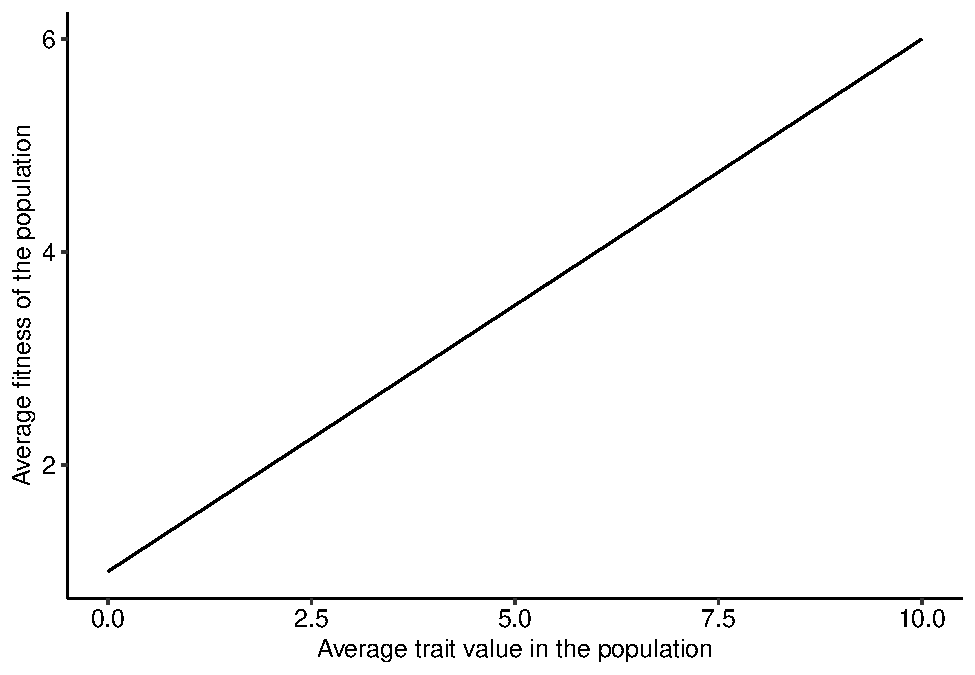
\includegraphics[width=0.65\linewidth,height=0.65\textheight]{_main_files/figure-latex/unnamed-chunk-18-1}

Now that we have the adaptive landscape, try to think about its shape and how evolution proceeds when we use the first fitness function. Your task for this section will be to adapt the code to simulate the evolutionary dynamics and the fitness landscape when we use the second fitness function, \(e^{-\alpha\left[\left(\theta-\overline{z}\right)^2 + \sigma^2\right]}\). Use both the function and the selection gradient, \(2\alpha (\theta-\overline{z})\), to simulate the adaptive landscape and the evolutionary dynamics of the trait. Try to answer the following questions:

\begin{enumerate}
\def\labelenumi{\arabic{enumi}.}
\item
  For both fitness functions, is there and end point to the evolutionary dynamics? If it does so, what would be this end point?
\item
  From the shape of the adaptive landscapes, could you predict how evolution would proceed in the population?
\item
  What sources of selective pressures and biological mechanisms could lead to these two adaptive landscapes and their underlying evolutionary dynamics?
\end{enumerate}

\hypertarget{exercise-simulating-coevolution-mediated-by-a-gene-for-gene-or-matching-allele-mechanisms}{%
\chapter{Exercise: Simulating coevolution mediated by a gene-for-gene or matching allele mechanisms}\label{exercise-simulating-coevolution-mediated-by-a-gene-for-gene-or-matching-allele-mechanisms}}

\hypertarget{simulating-coevolution-of-victim-exploiter-interactions}{%
\section{Simulating coevolution of victim-exploiter interactions}\label{simulating-coevolution-of-victim-exploiter-interactions}}

In first lecture of the second block we studied how we can use Wright's equation to model the gene-for-gene or matching allele coevolution of two interacting species. Particularly, we studied the example in which one of the species is an exploiter and benefit from the interaction, while the other is a victim that is negatively affected by the interaction. Here, we will perform numerical simulations of this coevolutionary model to gain intuition about how different assumptions about the mechanism of coevolution and types of interaction can change the outcome of the coevolutionary dynamics. We will begin with the gene-for-gene model with one exploiter and one victim species. In this model, we assumed that the interaction between a victim and exploiter depends on two components. First, it depends on a matrix describing how individuals carrying alleles \(A_{x}\) or \(B_{x}\) of the victim species are affected by the individuals carrying alleles \(A_{y}\) or \(B_{y}\) of the exploiter species:

\[
\begin{array}{cc} &
\begin{array}{cc} A_{y} && B_{y} \end{array}
\\
\begin{array}{cc}
A_{x} \\
B_{x} \end{array}
&
\left(
\begin{array}{cc}
\alpha_{AxAy} & \alpha_{AxBy} \\
\alpha_{BxAy} & \alpha_{BxBy} \end{array}
\right)\end{array}
\]

Second, it depends on the frequency of individuals carrying alleles \(A\) and \(B\) in the populations of the victim - \(p_{x}\) and \((1-p_{x})\) - and exploiter species - \(p_{y}\) and \((1-p_{y})\). Using these two components, the fitness consequences of ecological interactions for the individuals of the victim and exploiter species carrying either the \(A\) or \(B\) alleles are given by the following set of equations:

\[\begin{aligned}
W_{A,x}&=1-s_{x}\left[\alpha_{AxAy}p_{y}+\alpha_{AxBy}(1-p_{y})\right] \\
W_{B,x}&=1-s_{x}\left[\alpha_{BxAy}p_{y}+\alpha_{BxBy}(1-p_{y})\right] \\
W_{A,y}&=1+s_{y}\left[\alpha_{AyAx}p_{x}+\alpha_{AyBx}(1-p_{x})\right] \\
W_{B,y}&=1+s_{y}\left[\alpha_{ByAx}p_{x}+\alpha_{ByBx}(1-p_{x})\right] \\
\end{aligned}\]

where \(s_{x}\) and \(s_{y}\) are parameters that scale how strongly interactions affect fitness. Then, we can plug in these fitness functions into Wright's equation to obtain the recursive ones describing how the frequency of alleles change in both the victim and exploiter populations, as follows:

\[\begin{aligned}
p_{x}^{(t+1)}&=p_{x}^{(t)}+p_{x}^{(t)}(1-p_{x}^{(t)})\frac{\left(W_{A,x}^{(t)}-W_{B,x}^{(t)}\right)}{\overline{W}_{x}^{(t)}} \\
p_{y}^{(t+1)}&=p_{y}^{(t)}+p_{y}^{(t)}(1-p_{y}^{(t)})\frac{\left(W_{A,y}^{(t)}-W_{B,y}^{(t)}\right)}{\overline{W}_{y}^{(t)}}\end{aligned}\]

In the lecture, we substituted the values of fitness in the equation above using the assumptions that coevolution is mediated by a gene-for-gene mechanism. Here there is no need to do this, since it will be more convenient to directly implement the equations above in the simulation. To perform the numerical simulations we will follow the same steps as in the first exercise section, the only difference being that now we have two coupled equations. Once more, we will set up a \emph{for loop} to iterate over the equations and will go through the following steps:

\begin{enumerate}
\def\labelenumi{\arabic{enumi}.}
\item
  Define a function that takes as input parameters of the model, such as the matrix of effects, the maximum number of time steps of the model, and initial values of \(p_{x}\) and \(p_{y}\).
\item
  In a for loop, set the value of \(p_{x}\) and \(p_{y}\) to the one at the current time step, \(t\)
\item
  In a for loop, compute the average fitness of the populations as \(p_{x}W_{A,x}+(1-p_{x})W_{B,x}\) and \(p_{y}W_{A,y}+(1-p_{y})W_{B,y}\).
\item
  In a for loop, update the values of \(p_{x}\) and \(p_{y}\) using Wright's equation and our assumptions about the fitness consequences of interactions.
\item
  Return a data frame with the results.
\end{enumerate}

These steps are highlighted in the block of code below:

\begin{Shaded}
\begin{Highlighting}[]
\CommentTok{\# Step (1)}

\CommentTok{\#Defining a function that takes as input the following parameters:}

\CommentTok{\#A=Matrix of effects between alleles}
\CommentTok{\#sx=Overall strength of ecological interactions on fitness of the victim species}
\CommentTok{\#sy=Overall strength of ecological interactions on fitness of the exploiter species}
\CommentTok{\#p0\_x=Initial frequency of allele A of the victim species}
\CommentTok{\#p0\_y=Initial frequency of allele A of the exploiter}

\NormalTok{coevo}\OtherTok{\textless{}{-}}\ControlFlowTok{function}\NormalTok{(A, sx, sy, tmax, p0\_y, p0\_x)\{ }\CommentTok{\#Step (1)}
  
\NormalTok{x\_dp }\OtherTok{=} \FunctionTok{c}\NormalTok{() }\CommentTok{\#Creating vector to store values of the frequency of allele A for the victim species}
\NormalTok{y\_dp }\OtherTok{=} \FunctionTok{c}\NormalTok{() }\CommentTok{\#Creating vector to store values of the frequency of allele A for the exploiter species}

\NormalTok{x\_dp[}\DecValTok{1}\NormalTok{] }\OtherTok{=}\NormalTok{ p0\_x }\CommentTok{\#Setting initial frequency of allele A for the victim species}
\NormalTok{y\_dp[}\DecValTok{1}\NormalTok{] }\OtherTok{=}\NormalTok{ p0\_y }\CommentTok{\#Setting initial frequency of allele A for the exploiter species}

\CommentTok{\#For loop to iterate over the equation}
\ControlFlowTok{for}\NormalTok{(t }\ControlFlowTok{in} \DecValTok{1}\SpecialCharTok{:}\NormalTok{(tmax}\DecValTok{{-}1}\NormalTok{))\{}
  
  \CommentTok{\# Step (2)}
  
\NormalTok{  xp }\OtherTok{=}\NormalTok{ x\_dp[t] }\CommentTok{\#Setting current frequency of allele A for the victim species}
\NormalTok{  yp }\OtherTok{=}\NormalTok{ y\_dp[t] }\CommentTok{\#Setting current frequency of allele A for the exploiter species}
  
  \CommentTok{\# Step (3)}

\NormalTok{  x\_wA }\OtherTok{=} \DecValTok{1} \SpecialCharTok{{-}}\NormalTok{ sx}\SpecialCharTok{*}\NormalTok{(A[}\DecValTok{1}\NormalTok{,}\DecValTok{1}\NormalTok{]}\SpecialCharTok{*}\NormalTok{yp }\SpecialCharTok{+}\NormalTok{ A[}\DecValTok{1}\NormalTok{,}\DecValTok{2}\NormalTok{]}\SpecialCharTok{*}\NormalTok{(}\DecValTok{1}\SpecialCharTok{{-}}\NormalTok{yp)) }\CommentTok{\#Computing the fitness of allele A for the victim species}
\NormalTok{  x\_wB }\OtherTok{=} \DecValTok{1} \SpecialCharTok{{-}}\NormalTok{ sx}\SpecialCharTok{*}\NormalTok{(A[}\DecValTok{2}\NormalTok{,}\DecValTok{1}\NormalTok{]}\SpecialCharTok{*}\NormalTok{yp }\SpecialCharTok{+}\NormalTok{ A[}\DecValTok{2}\NormalTok{,}\DecValTok{2}\NormalTok{]}\SpecialCharTok{*}\NormalTok{(}\DecValTok{1}\SpecialCharTok{{-}}\NormalTok{yp)) }\CommentTok{\#Computing the fitness of allele B for the victim species}
\NormalTok{  x\_avg\_w }\OtherTok{=}\NormalTok{ xp}\SpecialCharTok{*}\NormalTok{x\_wA }\SpecialCharTok{+}\NormalTok{ (}\DecValTok{1}\SpecialCharTok{{-}}\NormalTok{xp)}\SpecialCharTok{*}\NormalTok{x\_wB }\CommentTok{\#Computing the average fitness of the population of the victim species}

\NormalTok{  y\_wA }\OtherTok{=} \DecValTok{1} \SpecialCharTok{+}\NormalTok{ sy}\SpecialCharTok{*}\NormalTok{(A[}\DecValTok{1}\NormalTok{,}\DecValTok{1}\NormalTok{]}\SpecialCharTok{*}\NormalTok{xp }\SpecialCharTok{+}\NormalTok{ A[}\DecValTok{2}\NormalTok{,}\DecValTok{1}\NormalTok{]}\SpecialCharTok{*}\NormalTok{(}\DecValTok{1}\SpecialCharTok{{-}}\NormalTok{xp)) }\CommentTok{\#Computing the fitness of allele A for the exploiter species}
\NormalTok{  y\_wB }\OtherTok{=} \DecValTok{1} \SpecialCharTok{+}\NormalTok{ sy}\SpecialCharTok{*}\NormalTok{(A[}\DecValTok{1}\NormalTok{,}\DecValTok{2}\NormalTok{]}\SpecialCharTok{*}\NormalTok{xp }\SpecialCharTok{+}\NormalTok{ A[}\DecValTok{2}\NormalTok{,}\DecValTok{2}\NormalTok{]}\SpecialCharTok{*}\NormalTok{(}\DecValTok{1}\SpecialCharTok{{-}}\NormalTok{xp)) }\CommentTok{\#Computing the fitness of allele B for the exploiter species}
\NormalTok{  y\_avg\_w }\OtherTok{=}\NormalTok{ yp}\SpecialCharTok{*}\NormalTok{y\_wA }\SpecialCharTok{+}\NormalTok{ (}\DecValTok{1}\SpecialCharTok{{-}}\NormalTok{yp)}\SpecialCharTok{*}\NormalTok{y\_wB }\CommentTok{\#Computing the average fitness of the population of the exploiter species}
  
  \CommentTok{\# Step (4)}
  
\NormalTok{  x\_dp[t}\SpecialCharTok{+}\DecValTok{1}\NormalTok{]}\OtherTok{=}\NormalTok{xp }\SpecialCharTok{+}\NormalTok{ ((xp}\SpecialCharTok{*}\NormalTok{(}\DecValTok{1}\SpecialCharTok{{-}}\NormalTok{xp)}\SpecialCharTok{*}\NormalTok{(x\_wA}\SpecialCharTok{{-}}\NormalTok{x\_wB))}\SpecialCharTok{/}\NormalTok{x\_avg\_w) }\CommentTok{\#Using Wright\textquotesingle{}s equaiton to compute frequency of A in the next generation for the victim species}
\NormalTok{  y\_dp[t}\SpecialCharTok{+}\DecValTok{1}\NormalTok{]}\OtherTok{=}\NormalTok{yp }\SpecialCharTok{+}\NormalTok{ ((yp}\SpecialCharTok{*}\NormalTok{(}\DecValTok{1}\SpecialCharTok{{-}}\NormalTok{yp)}\SpecialCharTok{*}\NormalTok{(y\_wA}\SpecialCharTok{{-}}\NormalTok{y\_wB))}\SpecialCharTok{/}\NormalTok{y\_avg\_w) }\CommentTok{\#Using Wright\textquotesingle{}s equaiton to compute frequency of A in the next generation for the exploiter species}
  
\NormalTok{\}}

\NormalTok{r}\OtherTok{=}\FunctionTok{data.frame}\NormalTok{(x\_dp, y\_dp, }\AttributeTok{t=}\DecValTok{1}\SpecialCharTok{:}\NormalTok{tmax) }\CommentTok{\# Step (5), creating a data frame with frequencies over time}

\FunctionTok{return}\NormalTok{(r)}
  
\NormalTok{\}}
\end{Highlighting}
\end{Shaded}

Now we have a function that simulate the coevolution of a victim and an exploiter species under any type of matrix of effects between alleles. Let's start simulating coevolution under a gene-for-gene mechanism. For the example of gene-for-gene coevolution that we studied in the lecture, the matrix takes the following form:

\[
\begin{array}{cc} &
\begin{array}{cc} A_{y} & B_{y} \end{array}
\\
\begin{array}{cc}
A_{x} \\
B_{x} \end{array}
&
\left(
\begin{array}{cc}
1 && 0 \\
1 && 1 \end{array}
\right)\end{array}
\]
Thus, we need to set up this matrix first, to pass it as an argument (the matrix \(A\) in the code) to our function. The code to do so is as follows:

\begin{Shaded}
\begin{Highlighting}[]
\CommentTok{\#Creating a 2x2 matrix with entries corresponding to the gene{-}for{-}gene one studied in the lecture}

\NormalTok{A}\OtherTok{=}\FunctionTok{matrix}\NormalTok{(}\AttributeTok{data=}\FunctionTok{c}\NormalTok{(}\DecValTok{1}\NormalTok{,}\DecValTok{1}\NormalTok{,}\DecValTok{0}\NormalTok{,}\DecValTok{1}\NormalTok{), }\AttributeTok{nrow=}\DecValTok{2}\NormalTok{, }\AttributeTok{ncol=}\DecValTok{2}\NormalTok{)}
\FunctionTok{rownames}\NormalTok{(A)}\OtherTok{=}\FunctionTok{c}\NormalTok{(}\StringTok{"Ax"}\NormalTok{, }\StringTok{"Bx"}\NormalTok{) }\CommentTok{\#Changing row names to facilitate visualization}
\FunctionTok{colnames}\NormalTok{(A)}\OtherTok{=}\FunctionTok{c}\NormalTok{(}\StringTok{"Ay"}\NormalTok{, }\StringTok{"By"}\NormalTok{) }\CommentTok{\#Changing column names to facilitate visualization}

\NormalTok{A}
\end{Highlighting}
\end{Shaded}

\begin{verbatim}
##    Ay By
## Ax  1  0
## Bx  1  1
\end{verbatim}

Now that we have the matrix of effects set up, we can pass it as an argument to the function that we developed earlier, along with other parameter values of the model. Then, we can run the function, and plot the results.

\begin{Shaded}
\begin{Highlighting}[]
\CommentTok{\#Running the coevolutionary model}
\NormalTok{r}\OtherTok{=}\FunctionTok{coevo}\NormalTok{(}\AttributeTok{A=}\NormalTok{A, }\AttributeTok{sx=}\FloatTok{0.1}\NormalTok{, }\AttributeTok{sy=}\FloatTok{0.1}\NormalTok{, }\AttributeTok{tmax=}\DecValTok{100}\NormalTok{, }\AttributeTok{p0\_y=}\FloatTok{0.2}\NormalTok{, }\AttributeTok{p0\_x=}\FloatTok{0.2}\NormalTok{)}

\CommentTok{\#Plotting the results}

\FunctionTok{library}\NormalTok{(ggplot2)}
\FunctionTok{library}\NormalTok{(ggpubr)}

\FunctionTok{ggplot}\NormalTok{()}\SpecialCharTok{+}
  \FunctionTok{geom\_line}\NormalTok{(}\AttributeTok{data=}\NormalTok{r, }\FunctionTok{aes}\NormalTok{(}\AttributeTok{x=}\NormalTok{t, }\AttributeTok{y=}\NormalTok{x\_dp), }\AttributeTok{color=}\StringTok{"royalblue3"}\NormalTok{)}\SpecialCharTok{+} \CommentTok{\# Frequency of allele A for victims, in blue}
  \FunctionTok{geom\_line}\NormalTok{(}\AttributeTok{data=}\NormalTok{r, }\FunctionTok{aes}\NormalTok{(}\AttributeTok{x=}\NormalTok{t, }\AttributeTok{y=}\NormalTok{y\_dp), }\AttributeTok{color=}\StringTok{"firebrick3"}\NormalTok{)}\SpecialCharTok{+} \CommentTok{\#Frequency of allele A for exploiters, in red}
  \FunctionTok{xlab}\NormalTok{(}\StringTok{"Generations"}\NormalTok{)}\SpecialCharTok{+}\FunctionTok{ylab}\NormalTok{(}\StringTok{"Frequency of allele A"}\NormalTok{)}\SpecialCharTok{+}
  \FunctionTok{theme\_pubr}\NormalTok{()}
\end{Highlighting}
\end{Shaded}

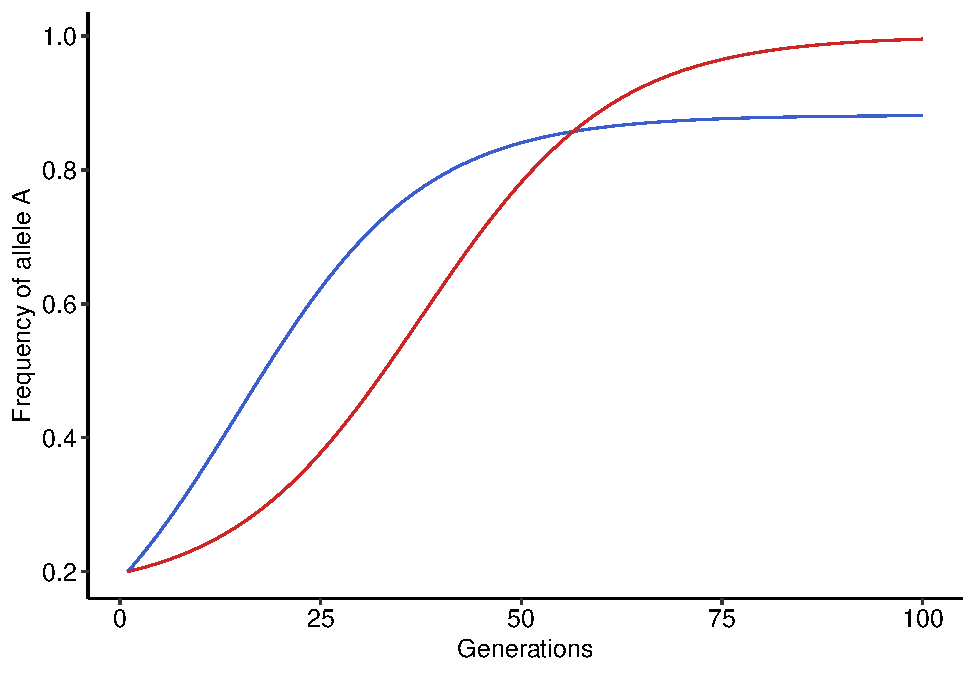
\includegraphics[width=0.65\linewidth,height=0.65\textheight]{_main_files/figure-latex/unnamed-chunk-21-1}

Using the function that simulates coevolution, try to explore how the coevolutionary dynamics changes under different parameter values. Try to answer the following questions:

\begin{enumerate}
\def\labelenumi{\arabic{enumi}.}
\tightlist
\item
  How different values of \(s_{x}\), \(s_{y}\) and initial frequency of alleles modify the outcome of coevolution?
\item
  Under what situations coevolution erodes polymorphism from the victim's population?
\end{enumerate}

\hypertarget{simulating-coevolution-of-antagonistic-interactions-under-different-assumptions}{%
\section{Simulating coevolution of antagonistic interactions under different assumptions}\label{simulating-coevolution-of-antagonistic-interactions-under-different-assumptions}}

Until now we are assuming that a gene-for-gene mechanism underlies the coevolution of victims and exploiters. However, in some cases the interaction may also depend on the matching of alleles, as in the interaction between the small crustacean \emph{Daphnia magna} and the bacteria \emph{Pasteuria ramosa} (Luijckx \emph{et al.} 2013). In this case, the matrix of effects takes the following form:

\[
\begin{array}{cc} &
\begin{array}{cc} A_{y} & B_{y} \end{array}
\\
\begin{array}{cc}
A_{x} \\
B_{x} \end{array}
&
\left(
\begin{array}{cc}
1 && 0 \\
0 && 1 \end{array}
\right)\end{array}
\]
Following our previous implementation, build this matrix in R and use it as an argument to simulate coevolution of a victim and an exploiter species under a matching allele mechanism. Plot the results and try to answer the following questions:

\begin{enumerate}
\def\labelenumi{\arabic{enumi}.}
\item
  What differences can you observe between the coevolutionary dynamics under a gene-for-gene or a matching allele mechanism?
\item
  What would be a possible explanation for these differences?
\end{enumerate}

\hypertarget{simulating-coevolution-of-mutualistic-interactions}{%
\section{Simulating coevolution of mutualistic interactions}\label{simulating-coevolution-of-mutualistic-interactions}}

In the previous section, we simulated coevolution of one victim and exploiter species under two different mechanisms determining the outcome of the interaction, gene-for-gene or matching allele. Here, we will slightly modify this coevolutionary model to encompass mutualistic interactions. To do so, we need to modify our assumption about how interactions affect the fitness of species, and what is the interaction mechanism mediating this effect. Mutualisms are interactions that increase the fitness of individuals. In that case, the equations for the fitness of individuals carrying the alleles A or B of two mutualists, are as follows:

\[\begin{aligned}
W_{A,x}&=1+s_{x}\left[\alpha_{AxAy}p_{y}+\alpha_{AxBy}(1-p_{y})\right] \\
W_{B,x}&=1+s_{x}\left[\alpha_{BxAy}p_{y}+\alpha_{BxBy}(1-p_{y})\right] \\
W_{A,y}&=1+s_{y}\left[\alpha_{AyAx}p_{x}+\alpha_{AyBx}(1-p_{x})\right] \\
W_{B,y}&=1+s_{y}\left[\alpha_{ByAx}p_{x}+\alpha_{ByBx}(1-p_{x})\right] \\
\end{aligned}\]

Since, many mutualistic interactions are mediated by a trait matching mechanism, we model this mechanism using the matrix of effects of the matching allele model:

\[
\begin{array}{cc} &
\begin{array}{cc} A_{y} & B_{y} \end{array}
\\
\begin{array}{cc}
A_{x} \\
B_{x} \end{array}
&
\left(
\begin{array}{cc}
1 && 0 \\
0 && 1 \end{array}
\right)\end{array}
\]
For this section, your task will be to adapt the function that simulate coevolution to incorporate the fitness equations and the matrix of effects for mutualisms. Then, simulate the coevolutionary dynamics and try to answer the following question:

\begin{enumerate}
\def\labelenumi{\arabic{enumi}.}
\item
  When mutualistic species coevolve, is it possible to maintain both alleles (i.e.~polymorphism) in the populations?
\item
  What would be a possible biological mechanism that could change this outcome? Think about a mechanism that we could include as an additional assumption in the fitness of individuals of the mutualistic species.
\end{enumerate}

  \bibliography{book.bib,packages.bib}

\end{document}
